\documentclass[12pt,a4paper]{report}
\usepackage{listings}

% Compatibilité Antidote
\usepackage[T1]{fontenc}
%\usepackage{lmodern}
\usepackage[numbers]{natbib} % do not declare this after babel

\usepackage[utf8]{inputenc}
\usepackage[francais]{babel}
\usepackage[colorlinks, linkcolor=blue]{hyperref}
\usepackage[all]{hypcap} % link lead on the top of the figure pictures
\usepackage{graphicx}
\usepackage[printonlyused,smaller]{acronym} %footnote,withpage
\usepackage{xcolor}
\usepackage{fancyvrb}
\usepackage{color}
\usepackage[margin=2.5cm]{geometry}
%\usepackage{fullpage}
\usepackage{makeidx}
\usepackage{pdfpages}
\usepackage{enumerate}
\usepackage{float}

% Declare color package and fix colortbl bug with tabular lines
\usepackage{color, colortbl}

\usepackage{array}
\newcolumntype{M}[1]{>{\arraybackslash}m{#1}}
\newcolumntype{N}{@{}m{0pt}@{}}


\usepackage{multirow}
\usepackage{multicol}
\hypersetup{citecolor = black, urlcolor = black, linkcolor= black} %pdfstartpage=4}

%\usepackage{tocbibind} % Table des matière dans la table des matières

\usepackage[babel=true]{csquotes} % csquotes va utiliser la langue définie dans babel
%\usepackage{cite}

\usepackage{fancyhdr}
\pagestyle{fancy}

\usepackage{subfigure}
%\setcounter{lofdepth}{2}
\usepackage[export]{adjustbox}

%\renewcommand{\chaptermark}[1]{\markboth{#1}{}}
\renewcommand{\chaptermark}[1]{%
  \ifnum\value{chapter}>0
    \markboth{Chapitre \thechapter{}~: #1}{}%
  \else
    \markboth{#1}{}%
  \fi
}

\fancyhead{} % clear all header fields
\fancyhead[RO,LE]{ %
	\ifnum\value{chapter}>0 \nouppercase{\leftmark}\fi
}
\fancyfoot{} % clear all footer fields
\fancyfoot[L]{\footnotesize\textsc{A. Python}}
\fancyfoot[R]{\thepage}
\renewcommand{\headrulewidth}{0.4pt}
\renewcommand{\footrulewidth}{0.4pt}


\fancypagestyle{plain}{ %
	\pagestyle{fancy}	
}

%\patchcmd{\chapter}{\thispagestyle{plain}}{\thispagestyle{fancy}}{}{}


% % % Définition de symboles et commandes % % %

\usepackage{xspace}
\newcommand{\formatac}[1]{%
\bgroup\renewcommand\acsfont{\textbf}%
\relax#1\relax\egroup\xspace}

% Texte entouré d'un rond
\newcommand{\rond}[1]{\textcircled{\scriptsize{#1}}}

% Référence à un élément (numéro et page)
\newcommand{\voir}[2]{(voir~#1 \ref{#2}, p.~\pageref{#2})}
\newcommand{\fnvoir}[2]{\footnote{#1 \ref{#2}, p.~\pageref{#2}}}

\newcommand{\fnurl}[2]{%
  \href{#2}{#1}\footnote{\url{#2}}%
}

% guillemets à la française (eg=entre guillemets)
\newcommand{\eg}[1]{\og{}#1\fg{}}


% Affiche plusieurs lignes d'un fichier à partir d'une ligne jusqu'à une autre avec lstinputlisting
\newcommand{\lstinputlines}[3]{\lstinputlisting[firstnumber=#1, firstline=#1, lastline=#2]{#3}}

% Affiche une seule ligne d'un fichier avec lstinputlisting
\newcommand{\lstinputline}[2]{\lstinputlines{#1}{#1}{#2}}


% Configuration du paquet listing
\lstset{
	language=C,
	extendedchars=true
	breaklines = true
	breakautoindent=true
	numbers = left
	stepnumber = 1
	numberstyle = \footnotesize
	keywordstyle=\color{blue}\bfseries\emph
	captionpos = b
	lstset{frame = tlrb}
	fancyvrb=false,
	basicstyle=\ttfamily\scriptsize,
	stringstyle=\ttfamily\color{green!50!black},
	directivestyle=\color{brown},
	keywordstyle=\color{blue}\bfseries,
	commentstyle=\color{red!50!black}\itshape,
	showspaces=false,
	showstringspaces=true,
	fontadjust=true,
	keepspaces=true,
%	flexiblecolumns=true % la propriété tabsize n'est pas respectée avec ce parapetre
	tabsize=2,
%	showtabs=true,
	frame=single,
	numbers=left, numberstyle=\tiny, firstnumber=1, stepnumber=1,
	numbersep=5pt,
	breaklines=true,
	escapeinside={(*@}{@*)},
	literate=%
		{ç}{{\c c}}1
		{Ç}{{\c C}}1
		{æ}{{\ae}}1
		{Æ}{{\AE}}1
		{œ}{{\oe}}1
		{Œ}{{\OE}}1
		{Å}{{\AA}}1
		{Å}{{\AA}}1
		{Â}{{\^A}}1
		{Ê}{{\^E}}1
		{Î}{{\^I}}1
		{Ô}{{\^O}}1
		{Û}{{\^U}}1
		{â}{{\^a}}1
		{ê}{{\^e}}1
		{î}{{\^i}}1
		{ô}{{\^o}}1
		{û}{{\^u}}1
		{á}{{\'a}}1
		{í}{{\'i}}1
		{é}{{\'e}}1
		{ý}{{\'y}}1
		{ú}{{\'u}}1
		{ó}{{\'o}}1
		{ě}{{\v{e}}}1
		{š}{{\v{s}}}1
		{č}{{\v{c}}}1
		{ř}{{\v{r}}}1
		{ž}{{\v{z}}}1
		{ď}{{\v{d}}}1
		{ť}{{\v{t}}}1
		{ň}{{\v{n}}}1                
		{ů}{{\r{u}}}1
		{Á}{{\'A}}1
		{Í}{{\'I}}1
		{É}{{\'E}}1
		{Ý}{{\'Y}}1
		{Ú}{{\'U}}1
		{Ó}{{\'O}}1
		{Ě}{{\v{E}}}1
		{Š}{{\v{S}}}1
		{Č}{{\v{C}}}1
		{Ř}{{\v{R}}}1
		{Ž}{{\v{Z}}}1
		{Ď}{{\v{D}}}1
		{Ť}{{\v{T}}}1
		{Ň}{{\v{N}}}1                
		{Ů}{{\r{U}}}1    
}

\usepackage{units}
%\usepackage{dirtree}
\usepackage{amsmath}
\usepackage{mathtools} % \shortintertext for comments in align
\usepackage{amssymb}
\usepackage{relsize}
\usepackage{calc}

\usepackage[inline]{enumitem}

\usepackage{eurosym}

\usepackage{tikz}
\usetikzlibrary{shapes,snakes}
\usetikzlibrary{backgrounds}

\usepackage{algorithm2e}
\usepackage{algorithmic}

\newcommand{\XLUPS}[1]{\textsc{\footnotesize #1}\acs{LUPS}}
\newcommand{\XFLUPS}[1]{\textsc{\footnotesize #1}\acs{FLUPS}}

%\makeindex
\begin{document}
%\newcommand{\HRule}{\rule{\linewidth}{0.5mm}}
\begin{titlepage}

\begin{minipage}{1\textwidth}
\hspace{-0.048\textwidth}  % fullpage default margin
%\hspace{-0.0795\textwidth} % geometry default margin
%\includegraphics[scale=0.147]{images/hepia.jpg}
\hspace{0.316\textwidth}
%\includegraphics[scale=0.0841]{images/hesso.jpg}
\end{minipage}

\begin{center}


%\usepackage{yfonts}
%{ \Huge
%\textswab{das DateiSystem}\\
%\textfrak{das DateiSystem}\\
%\textgoth{das DateiSystem}
%}

~\\[2.5cm]

% Title
%\HRule \\[0.4cm]
%{ \Huge \bfseries \includegraphics[scale=0.4]{images/dasDateiSystem.pdf}} \\[0.3cm]
%{ \Large \bfseries Dynamically Aggregated Storages File System\\[0.3cm]
% (avec le \textit{framework} FUSE)}\\[1.3cm]
{ \Large \bfseries Foo Bar Title}\\[1.3cm]
%\HRule \\[0.8cm]

{\Large Thèse de master en sciences informatiques}\\[0.5cm]
\textbf{\textit{Session 2017}}\\[1.5cm]



\includegraphics[scale=0.3]{images/placeholder.png} \\[2cm]
%\vfill


\end{center}

\begin{minipage}{8\textwidth}
\begin{flushleft} \large
\textbf{Professeur responsable:} \textsc{Latt}~Jonas\\
\textbf{Diplômant:} \textsc{Python}~Adrien
\end{flushleft}
\end{minipage}


\end{titlepage}

\pagenumbering{Roman}

\chapter*{Avant-propos}
%\addcontentsline{toc}{chapter}{Avant-propos}
\section*{Présentation}

\section*{Conventions typographiques}\label{title-avantpropos}

\noindent Ce document suit des règles typographiques afin d'en simplifier la lecture:

\begin{itemize}
\item l'\textit{italique} est employé pour les termes anglais ou sur lesquels l'attention est attirée;
\item une police de caractère à \texttt{chasse fixe} indique un extrait de code, une commande, un chemin ou la sortie standard d'une console.
\end{itemize}

\section*{Remerciements}

\tableofcontents

\cleardoublepage
% \phantomsection
%\addcontentsline{toc}{chapter}{\listfigurename}
\listoffigures


\chapter*{Acronymes}

\begin{acronym}[11222232]
%\acro{}{\href{}{}}

\acro{AoS}{Array of Structures}
\acro{ASCII}{\href{https://fr.wikipedia.org/wiki/American_Standard_Code_for_Information_Interchange}{American Standard Code for Information Interchange}}
\acro{CPU}{\href{https://fr.wikipedia.org/wiki/Processeur}{Central Processing Unit}}
\acro{CP}{Co-Processeur}
\acro{CS}{Collide \& Stream}
\acro{ECC}{\href{https://fr.wikipedia.org/wiki/Mémoire_à_code_correcteur_d'erreurs}{Error-correcting code}}
\acro{ELBM}{Entropic \acs{LBM}}
\acro{FLUPS}{Lattice Cell Update Per Second}
\acro{FMA}{\href{http://docs.nvidia.com/cuda/floating-point/\#fused-multiply-add-fma}{Fused Multiply-Add}}
\acro{GPU}{\href{https://fr.wikipedia.org/wiki/Processeur_graphique}{Graphics Processing Unit}}
\acro{IDE}{\href{https://fr.wikipedia.org/wiki/Environnement_de_d\%C3\%A9veloppement}{Environnement de développement Intégré}}
\acro{LBM}{\href{https://fr.wikipedia.org/wiki/Méthode_de_Boltzmann_sur_réseau}{Lattice Boltzmann Method}}
\acro{LUPS}{Lattice Update Per Second}
\acro{MPI}{\href{https://fr.wikipedia.org/wiki/Message_Passing_Interface}{Message Passing Interface}}
\acro{SM}{Streaming Multiprocessor}
\acro{SoA}{Structure of Arrays}
\acro{SP}{Stream Processor}
\end{acronym}

\chapter{Introduction}
\pagenumbering{arabic}
La simulation de fluide numérique a de nombreuses applications dans domaines aussi varié que la géologie pour l'étude des volcans \cite{brogi_lattice_2017}, du jeux-vidéo pour un rendu réaliste de l'eau, du médical pour modéliser l'écoulement du sang \cite{hirabayashi_lattice_2004}, de l'aviation pour étudier l'aérodynamisme d'un fuselage et en prédire le bruit \cite{lew_noise_2010}, et bien autres encore. C'est par conséquent un sujet qui intéresse de nombreux chercheurs.

La méthode de Lattice Boltzmann (\acf{LBM} en anglais) est un algorithme de simulation de fluide attractive pour sa disposition à modéliser des comportements de fluides complexes et à être parallélisé.

Palabos, un solveur en mécanique des fluides numérique basé sur \acs{LBM}, permet de distribuer la simulation sur un \textit{cluster} de \acs{CPU} pour accélérer les calculs. Cette parallélisation pourrait encore être poussée  davantage pour certaines parties du domaine en les calculant sur \acs{GPU}. En effet, ces derniers se prêtent particulièrement bien aux algorithmes parallèles.

C'est là l'objectif de ce travail qui propose une implémentation de \acs{LBM} sur \acs{GPU}, réalisée pour Palabos afin, d'en améliorer les performances.

Après une vue d'ensemble des méthodes utilisées dans la simulation de fluide avec \acs{LBM}, ce document présente ensuite l'implémentation réalisée à travers ses deux principales phases de développement; la réalisation du code \acs{GPU} puis son intégration à Palabos.
Le document discute ensuite des performances mesurées pour estimer les capacités de l'implémentation, et propose finalement son modèle de performance.


\chapter{Méthode de Lattice Boltzmann}

\section{Algorithme} \label{title-lbm_algo}
Pour simuler le comportement de fluides, \acs{LBM} découpe l'espace physique à modéliser en un domaine discret composé de populations, organisées en une grille, et discrétise le temps en générations. 

Une population représente une portion de l'espace physique. Une simulation consiste en l'application de deux étapes de calculs, effectuées de façon identique sur chaque population du domaine, pour calculer celui de la génération suivante où le processus pourra être répété. Le résultat de la génération $t$ ne dépend par conséquent que de l'état du domaine à la génération $t-1$.  Il s'agit, à l'instar du bien connu jeu de la vie de \textsc{J.~Conway}, d'un automate cellulaire.


Une population, illustrée par les figures \ref{fig:population_d2q9}, est composée de 9 directions (nord, sud, est ...), auxquelles sont attribuées une valeur qui représente la densité de probabilité qu'a la vélocité du fluide d'aller dans une direction donnée.

\begin{figure}[h]
	\centering
	\subfigure[Directions]{%
		\centering
		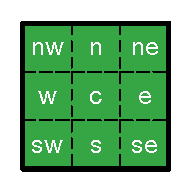
\includegraphics[scale=1]{images/population.pdf}
	}
	\subfigure[Numérotation]{%
		\centering
		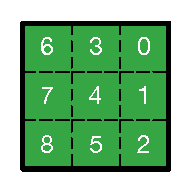
\includegraphics[scale=1]{images/population_numerotation.pdf}
	}
	\caption{Population D2Q9}
	\label{fig:population_d2q9}
\end{figure}
Les populations du domaine sont notées $f^{in}(x,t) = \{f^{in}_0(x,t), f^{in}_1(x,t), \dots f^{in}_8(x,t)\}$, avec $x$ la position dans la grille.

La première étape de simulation d'une génération, dite de \textit{collision}, introduit les vecteurs de vélocité $v$,  tel que les voisins de $f^{in}(x, t)$ sont trouvés par $f^{in}(x+v_i,t)$: 
\begin{multicols}{3}
\begin{itemize}
\item[] $v_0 = [1,1]$
\item[] $v_1 = [1,0]$
\item[] $v_2 = [1,-1]$
\item[] $v_3 = [0,1]$
\item[] $v_4 = [0,0]$
\item[] $v_5 = [0,-1]$
\item[] $v_6 = [-1,1]$
\item[] $v_7 = [-1,0]$
\item[] $v_8 = [-1,-1]$
\end{itemize}
\end{multicols}

On commence par calculer les variables \textit{macroscopiques} de la population, soit sa densité $\rho$ et ses vélocités $u$:\\[-2\baselineskip]
\begin{multicols}{2}
\begin{equation}
\rho(x, t) = \sum_{i=0}^{8} f^{in}_i(x,t)
\end{equation}
\begin{equation}
u = \frac{1}{\rho(x,t)}\sum_{i=0}^{8} v_i \cdot f^{in}_i(x,t)
\end{equation}
\end{multicols}~\\[-0.5\baselineskip]
\noindent puis on calcule les directions $i$ de la population $f^{out}$ qui résultent de la collision:
\begin{equation}
f^{out}_i = f^{in}_i - \omega \cdot \big(f^{in}_i - E(i, \rho, u) \big)
\end{equation}\\[-\baselineskip]

\noindent avec $E$ la fonction d'\textit{equilibrium}:
\begin{equation}
E(i, \rho, u) = \rho\cdot t_i \bigg(  1 + \frac{v_i \cdot u}{c^2_s} + \frac{1}{2~c^4_s} (v_i \cdot u)^2 - \frac{1}{2~c^2_s} |u|^2 \bigg)
\end{equation}\\[-\baselineskip]

\noindent avec $c_s$ la vitesse du son, $\omega$ le paramètre de relaxation, et $t_i = \nicefrac{1}{9}$ pour les directions orthogonales, et les constantes $t_i$, qui compense les longueurs inégales des différentes vélocités, avec $t_i =\nicefrac{1}{36}$ pour les diagonales et $t_i=\nicefrac{4}{9}$ pour la centrale, soit $t = \{\nicefrac{1}{36} , \nicefrac{1}{9}, \nicefrac{1}{36}, \nicefrac{1}{9}, \nicefrac{4}{9}, \nicefrac{1}{9}, \nicefrac{1}{36}, \nicefrac{1}{9}, \nicefrac{1}{36}\}$.

La seconde étape, illustrée par les figures \ref{fig:population_streaming}, propage les densités des populations $f^{out}$ calculées dans cette génération $t$ dans les nouvelles populations de la suivante $t+\delta t$, où $\delta t$ correspond au pas de temps utilisé.

\begin{equation}
f^{in}_i(x,t) = f^{out}_i(x-v_i\delta t, t - \delta t)
\end{equation}

On observe dans ce processus qu'il est hautement parallélisable. Chaque population est calculée indépendamment des autres jusqu'à la propagation qui elle n'implique que les voisins directs de la cellule. C'est ce potentiel qu'exploitent les implémentations les plus performantes, pour accélérer leur simulation.

\begin{figure}[h]
	\centering
	\subfigure[Génération $t$]{%
		\centering
		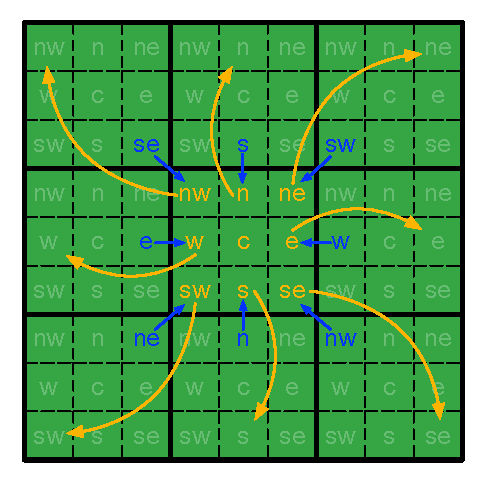
\includegraphics[scale=0.8995]{images/pre-streaming.pdf}
	}
	\subfigure[Génération $t+\delta t$]{%
		\centering
		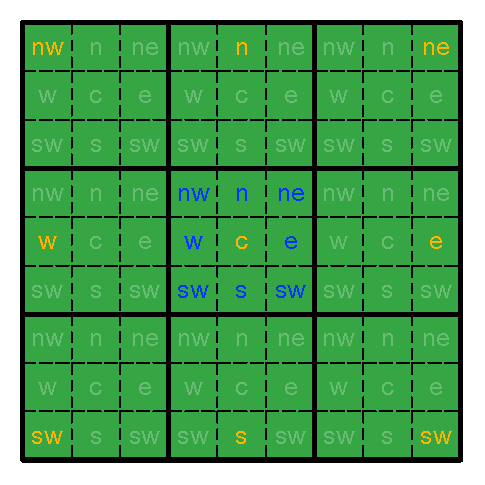
\includegraphics[scale=0.8995]{images/post-streaming.pdf}
	}
	\caption{Propagation pour la population $f^{in}(x,t)$ au centre ($x=[1,1]$) }
	\label{fig:population_streaming}
\end{figure}

\section{Notation DnQm}
L'algorithme présenté dans la section \ref{title-lbm_algo} est axé sur un domaine en 2 dimensions, et avec des populations à 9 directions. On note cette configuration D2Q9, avec D2 pour le nombre de dimensions et $Q9$ le nombre de directions. 

En effet, l'algorithme est également généralisé pour 3 dimensions, avec les configurations D3Q15, D3Q19 et D3Q27.

\section{Unité de mesure de performance LUPS}

La simulation de fluide avec \acs{LBM} est un processus gourmand en mémoire et temps de calcul. Un pan important de la recherche concernant \acs{LBM} vise à trouver des techniques pour améliorer les performances de son implémentation.

Les \acl{LUPS} (populations calculées par seconde) ou \XLUPS{} sont communément utilisés à cette fin.

\chapter{État de l'art}\label{title-sota}
\acs{LBM} est un algorithme propice pour des simulations distribuées sur les nœuds d'un \textit{cluster} de calcul, ou sur les cœurs d'un \acs{GPU}. Il a par conséquent attiré l'attention de nombreux chercheurs. 

Ce chapitre fait un tour d'horizon des technologies et des méthodes utilisées pour améliorer les performances des simulations basées sur la méthode de Lattice Boltzmann. Les sections suivantes présentent les travaux chronologiquement, en commençant par les simulations réalisées sur les processeurs Cell, puis les travaux qui utilisent les \acs{CPU} comme puissance de calcul. Sont ensuite  observées les recherches axées sur le portage de cet algorithme sur \acs{GPU} et finalement les méthodes de simulation hybrides entre \acs{CPU} et \acs{GPU}.

Les articles discutés ici se concentrent, pour la plupart, sur les implémentations D3Q19, mais d'autres configurations sont abordées et sont alors spécifiées.

\section{Simulations sur processeurs Cell}
Cell est un processeur multi-core développé par Sony, Toshiba et IBM à partir de 2001. Ces processeurs, optimisés pour le calcul parallèle, équipent notamment la console de jeu PlayStation3, mais aussi certains super-ordinateurs.\\

\citet{peng_parallel_2008} comparent en \citeyear{peng_parallel_2008} les performances d'un code \acs{LBM} sur un \textit{cluster} de neuf consoles PlayStation3 avec celles d'un \textit{cluster} Xeon classique. Pour l'étape de collision, ils observent que les PlayStation3 dépassent les performances des Xeon pour les problèmes plus grands que 1024 et qu'elles s'améliorent plus le domaine est grand. L'étape de propagation marque de meilleures performances sur le \textit{cluster} de PlayStation3 pour les domaines plus grands que 2048. En effet, cette étape est surtout intensive au niveau des communications. Or, la bande passante Ethernet (plutôt bas prix) de la PlayStation3 est moins bonne que celle d'un \textit{cluster} Xeon.

Au final, les auteurs observent des performances jusqu'à 11.02 fois meilleures avec les processeurs Cell de la PlayStation3 que sur un cluster Xeon, avec le domaine de simulation le plus grand. À titre de comparaisons, une seconde implémentation Cuda est réalisée et affiche un \textit{speed-up} de 8.76 par rapport au \acs{CPU}.\\

\citet{sturmer_fluid_2009} présentent en \citeyear{sturmer_fluid_2009} un solveur \acs{LBM} sur processeur Cell pour l'étude des anévrismes. En effet, il est très difficile, si ce n'est impossible, de mesurer avec précision les paramètres hémodynamiques dans les artères intracrâniennes d'un patient vivant. Une simulation sur PlayStation3 offre une solution pour la compréhension du développement des anévrismes, et de leur ruptures, qui se révèle abordable pour l'hôpital qui l'utilise (la console étant vendue à 400\euro~à l'époque).

En plus de son prix avantageux, de ses dimensions compactes qui permettent d'installer le dispositif n'importe où, et de sa faible consommation d'énergie, les auteurs affirment que la PlayStation3 dépasse par un facteur de 3.7 les performances d'un Intel Xeon 5160, avec la solution développée.\\

\citet{biferale_lattice_2010} réalisent en \citeyear{biferale_lattice_2010} une implémentation \acs{LBM} D2Q37 (figure~\ref{fig:d2q37})  pour QPACE, un super-ordinateur massivement parallèle basé sur des processeurs PowerXCell~8i.
Les simulations réalisées étudient les propriétés de l'instabilité de Rayleigh–Taylor sur de grands domaines de $4096\times 6000$ et $2048\times 3600$ populations, sur respectivement $2.6\cdot 10^5$ et $10^6$ générations pour des temps d'exécution de 32 et 44 heures par simulation. 
Les auteurs notent vis-à-vis de l'implémentation que leur routine de collision est la plus gourmande en temps d'exécution, en raison des calculs de nombres flottants, et que la propagation constitue le goulot d'étranglement de plus important de l'implémentation, en raison de la trop faible bande passante de $\sim 3.5$ Go/s.

\begin{figure}[h]
	\centering
	\includegraphics[scale=1, page=2, trim=68 522 340 80,clip]{../../Master-Thesis/doc/Articles/LBM/Cell/Biferale-2010.pdf}
	\caption{Population D2Q37 telle qu'illustrée par \citet{biferale_lattice_2010}}
	\label{fig:d2q37}
\end{figure}

\citet{williams_lattice_2008} développent en \citeyear{williams_lattice_2008}  un ensemble d'optimisations pour LBMHD (une application \acs{LBM} pour modéliser les turbulences magnétohydrodynamiques) appliquées automatiquement par un générateur de code, qui crée plusieurs versions du code (par optimisation appliquée) pour les architectures multi-core Intel Clovertown, AMD Opteron X2, Sun Niagara2, STI Cell et Intel Itanium2. Les codes sont ensuite auto-évalués pour déterminer les optimisations les plus intéressantes par plateforme.

Les auteurs observent que le processeur Cell offre très nettement les meilleures performances, mais déplorent la difficulté de développer pour ce matériel (éloigné des pratiques de programmation classiques). Ils soulignent également le succès de leur méthode d'\textit{auto-tuning} du code qui parvient à des \textit{speed-up} allant jusqu'à 14 fois les performances du code original.

\section{Simulations sur \acs{CPU}}
Si les processeurs de type Cell ont un temps offert une alternative intéressante aux \acs{CPU} pour accélérer les calculs parallèles, ces derniers restent pourtant toujours une unité de calcul très utilisée de nos jours.\\

\citet{min_performance_2013} exécutent en \citeyear{min_performance_2013} des \textit{benchmarks} pour le programme de simulation \acs{LBM} distribuée Palabos, sur le super-ordinateur chinois Sunway BlueLight MPP (le deuxième super-ordinateur le plus puissant de Chine en 2011). Ils décrivent dans leur article l'utilisation novatrice des \textit{flags} (standard) d'optimisation pour la compilation les sources de Palabos, à savoir \texttt{optimize = true}, \texttt{MPIparallel=true}, \texttt{optimFlags=-O3 -OPT:Ofast} et la définition des compilateurs SW1600 \texttt{serialCC=swCC} et \texttt{parallelCXX=mpiswCC}.

Ils comparent ensuite dans leurs mesures les performances relevées pour différents nombres de \textit{cores} utilisés et relèvent que leur stratégie d'exécution parallèle et d'optimisation réduit le temps d'exécution (par rapport à une exécution séquentielle et non-optimisée).\\

En \citeyear{li_parallelizing_2016}, \citet{li_parallelizing_2016} optimisent des exécutions parallèles de l'implémentation D3Q19 du programme open-source \textit{openlbmflow} sur Tianhe-2, le super-ordinateur chinois le plus puissant de l'époque. Cette machine est composée de 16000 nœuds de calculs, chacun muni de deux processeurs Xeon E5-2692 v2 et trois Xeon Phi 31S1P MIC.

Les auteurs exploitent les capacités du \textit{cluster} à travers des exécutions hybrides sur ces deux types de processeurs. Pour tirer les meilleures performances de cette collaboration, ils optimisent l'utilisation de la cache et de l'architecture SIMD, utilisent une implémentation hybride entre MPI et OpenMP pour la parallélisation et un système de \textit{load-balancing} entre les deux types de processeurs, pour éviter des transferts de données inutiles.

Sur un seul nœud de calcul, l'implémentation affiche jusqu'à un \textit{speed-up} de 3.2 avec l'approche collaborative, par rapport à une exécution n'utilisant que les deux \acs{CPU} du nœud. Les mesures d'exécutions sur de nombreux nœuds montrent quant à eux une bonne capacité de montée en charge de l'approche hybride.\\

En \citeyear{schmieschek_lb3d_2017}, \citet{schmieschek_lb3d_2017} présentent leur optimisation de l'implémentation \textit{open-source} LB3D qu'ils ont ensuite testé sur le super-ordinateur ARCHER au Royaume-Uni. 
Afin de vérifier que le \textit{refactoring} opéré n'a pas compromis le fonctionnement d'origine de LB3D, les auteurs ont réalisé des simulations de décomposition spinodale d'un mélange amphiphile, de détermination de la perméabilité d'un modèle en milieu poreux et enfin de la formation de mésophases amphiphiles. 

Les simulations réalisées sur ARCHER montrent un \textit{speedup} de 3 par rapport à la version non optimisée et permettent d'observer une excellente montée en charge jusqu'à 49152 \textit{cores} vers lesquels les performances commencent à se détériorer.

\section{Simulations sur \acs{GPU}}
L'évolution des capacités de calcul des \acs{GPU}, qui dépassent désormais largement celles des \acs{CPU}, ne passe pas inaperçue aux yeux des chercheurs, qui au début des années 2000 commencent à en explorer les capacités pour \acs{LBM} \cite{bolz_sparse_2003, buck_brook_2004, kruger_linear_2003}. En effet, cette technologie offre des performances grandissantes d'année en année, à un prix raisonnable. Une tendance soutenue en 2007 avec l'arrivée de CUDA, une technologie qui permet de programmer en C les \acs{GPU} de Nvidia.\\

\citet{li_implementing_2003} proposent ainsi en \citeyear{li_implementing_2003} une implémentation qu'ils testent sur une GeForce4 Ti 4600 et comparent les performances avec une implémentation \acs{CPU} sur un PC avec un processeur P4 1.6GHz et 512MB de mémoire DDR. 
Ils observent un \textit{speed-up} de 50 par rapport à la version \acs{CPU}, à partir d'un domaine de dimension $32^3$. Les performances alors atteintes, d'environ 9.8~\XLUPS{M}  pour un domaine de $256^3$, permettent de visualiser interactivement la simulation, notamment des domaines de $64^3$ et $128^3$.\\

\citet{toelke_teraflop_2008} implémentent en \citeyear{toelke_teraflop_2008}  un modèle D3Q13 avec la technologie CUDA, publiée un an plus tôt. Ils en explorent et expliquent brièvement le fonctionnement, avant de détailler celui de leur implémentation. Les mesures, réalisées avec une GeForce 8800, affichent des performances allant jusqu'à 592~\XLUPS{M}  en simple précision.\\

\citet{kaufman_implementing_2009} publient en \citeyear{kaufman_implementing_2009} leurs mesures de performances obtenues avec quatre implémentations interactives sur \acs{GPU} qu'ils comparent à des simulations similaires sur \acs{CPU}. 

La première est programmée avec Cg (un langage développé par Nvidia et Microsoft) et OpenGL, en simple précision. Testée sur une GeForce FX 5900 Ultra (cadencé à 400~MHz avec 256MB de DDR SDRAM), elle atteint les 3.87~\XLUPS{M}  sur un domaine de dimensions $128^3$, soit un \textit{speed-up} de 17 par rapport à une implémentation \acs{CPU} sur un Pentium IV (cadencé à 2.53 GHz avec 1 GB de PC800 RDRAM).

La seconde simule un domaine $480 \times 400 \times 80$ sur un \textit{cluster} de \acs{GPU} (GeForce FX 5900 Ultra) où chaque nœud calcule un sous-domaine $80^3$. Elle parvient à 51.68~\XLUPS{M}  sur 32 nœuds, contre 11.38~\XLUPS{M}  avec un \textit{cluster} de \acs{CPU} (Interl Pentium Xeo 2.4 GHz).

La troisième utilise Zippy, un \textit{framework} qui simplifie le développement d'application pour \textit{cluster} de \acs{GPU}. Les simulations, réalisées avec la même configuration que celle du paragraphe précédent, atteignent les 80~\XLUPS{M} sur un \textit{cluster} de \acs{GPU} Nvidia Quadro FX 4500 et de \acs{CPU} Intel Xeon 3.6 GHz.

Finalement, la troisième implémentation, réalisée avec CUDA, atteint les 144~\XLUPS{M}  sur une Nvidia Quadra FX 4600 sur un domaine $64^3$ (contre 94~\XLUPS{M}  avec Zippy sur cette même carte) et 278~\XLUPS{M}  sur un domaine $96^3$ avec une Nvidia Tesla C1060. Avec cette carte, les performances de cette dernière simulation chutent à 121~\XLUPS{M}  en double précision.\\

La même année, \citet{bailey_accelerating_2009} présentent une implémentation CUDA et discutent des optimisations réalisées (notamment vis-à-vis de l'accès à la mémoire globale du \acs{GPU}) pour en améliorer les performances. Ils les mesurent ensuite sur une Nvidia 8800 GTX sur laquelle ils relèvent 300~\XLUPS{M} en simple précision. Ceci correspond à un \textit{speed-up} de 28 par rapport à une simulation sur \acs{CPU} Intel quadcore d'une implémentation utilisant OpenMP (une interface de programmation parallèle). 

Les auteurs relèvent par ailleurs que CUDA permet une utilisation plus précise des ressources matérielles du \acs{GPU} par rapport aux autres interfaces de programmation OpenGL, Rapidmind et BrookGPU.\\

\citet{kuznik_lbm_2010} présentent en \citeyear{kuznik_lbm_2010} une implémentation D2Q9 en CUDA sur laquelle ils mesurent notamment l'influence sur les performances des nombres flottants en simple et double précision. Si leur implémentation atteint les 915~\XLUPS{M}  avec un domaine $2048^2$ sur une Nvidia GTX280, les performances tombent à 239~\XLUPS{M}  en double précision, soit d'un facteur 3.8.\\

\citet{rinaldi_lattice-boltzmann_2012} proposent en \citeyear{rinaldi_lattice-boltzmann_2012} une implémentation CUDA sur laquelle ils relèvent l'importance pour les performances qu'occupent les accès \textit{coalesced} à la mémoire globale, son schéma d'accès, l'utilisation de la mémoire partagée et la réduction du nombre de branchements (\texttt{if}/\texttt{else}).

Ils mesurent ensuite les performances de leur implémentation qui atteignent 259~\XLUPS{M} sur une Geforce GTX 260. Des optimisations supplémentaires, comme l'utilisation de constante à la place de paramètres d'exécution et la réduction du nombre d'\textit{output} entre les itérations, permettent d'atteindre 400~\XLUPS{M}, au prix d'une flexibilité et précision réduite.\\

La même année, \citet{astorino_modular_2012} présentent leurs implémentations D3Q15 et D3Q19 avec lesquelles ils atteignent respectivement 490~\XLUPS{M} et 370~\XLUPS{M} sur une GeForce GTX 480.

Parmi les optimisations exposées, leur article analyse les arrangements mémoires \acs{AoS} (\acl{AoS}) et \acs{SoA} (\acl{SoA}), illustré par la figure~\ref{fig:aos_soa}.

\begin{figure}[h]
	\centering
	\subfigure[Array-of-Structures]{%
		\centering
		
\includegraphics[scale=1, page=11, trim=101 580 324 160,clip]{../../Master-Thesis/doc/Articles/LBM/GPU/Astorino-2011.pdf}
		\label{fig:aos}
	}
	\subfigure[Structure-of-Arrays]{%
		\centering
		
\includegraphics[scale=0.97, page=11, trim=324 580 100 160,clip]{../../Master-Thesis/doc/Articles/LBM/GPU/Astorino-2011.pdf}
		\label{fig:soa}
	}
	\caption{Arrangements mémoire \acs{AoS} et \acs{SoA} tels qu'illustrés par \cite{astorino_modular_2012}}
	\label{fig:aos_soa}
\end{figure} 

\acs{AoS} conserve les structures de populations $f_i(x)$ les unes à côté des autres, soit leurs directions $i = \{1\dots Q\}$ avec Q le nombre de directions (9 en D2Q9, 19 en D3Q19, ...) et N la taille du domaine:
\begin{equation*}
f_{\acs{AoS}} = f_1(1), f_2(1), \dots f_Q(1), f_1(2), f_2(2), \dots f_Q(2), \dots f_1(N), f_2(N), \dots f_Q(N)
\end{equation*}

\noindent tandis qu'\acs{SoA} conserve les \eg{tableaux} de populations avec les cellules côte à côte:
\begin{equation*}
f_{\acs{SoA}} = f_1(1), f_1(2), \dots f_1(N), f_2(1), f_2(2), \dots f_2(N), \dots f_Q(1), f_Q(2), \dots f_Q(N)
\end{equation*}

Ces deux arrangements optimisent des étapes différentes. En effet, \acs{AoS} est efficace lors de la collision, qui accède simultanément aux directions de la cellule $x$, tandis que \acs{SoA} est optimisé pour la propagation, qui accède aux cellules voisines de $x$, une direction après l'autre. C'est cet arrangement qu'utilise l'implémentation que présentent les auteurs.\\

\citet{habich_performance_2013} publient en \citeyear{habich_performance_2013} une comparaison entre les performances de leurs implémentations CUDA et OpenCL sur une carte Nvidia Tesla C2070 et AMD 6970. Ils commencent par mesurer l'effet de l'utilisation d'une mémoire \acs{ECC} (\acl{ECC} memory) et notent une baisse des performances de 10 à 18\% lorsqu'elle est activée.

Les deux implémentations affichent les mêmes performances sur les deux cartes avec 650~\XLUPS{M} en simple précision et 290~\XLUPS{M} en double précision.\\

\citet{januszewski_sailfish_2014} présente Sailfish en \citeyear{januszewski_sailfish_2014}, une implémentation multi-\acs{GPU} en Python de \acs{LBM}. Cette dernière utilise une approche novatrice, dans le sens qu'elle génère au \textit{run-time} le code CUDA ou OpenCL qu'elle exécute ensuite sur \acs{GPU}. Sailfish profite ainsi de l'expressivité et de la flexibilité du langage Python pour la configuration des simulations et de la puissance de calcul des \acs{GPU} offerte par l'utilisation de CUDA ou OpenCL.

La figure~\ref{fig:sailfish_perf} illustre les mesures de performances réalisées par les auteurs, avec un code généré en CUDA sur un domaine $256 \times 100\times 100$, en simple et double précision, en D3Q13, D3Q15, D3Q19 et D3Q27 sur 6 cartes graphiques différentes.

\begin{figure}[h]
	\centering
	\subfigure[Simple précision]{%
		\centering
		\begin{tikzpicture}[scale=1]
		\clip (2.01,0.5)--(2.2,0.5)--(2.2,-0.5)--(-4.1,-0.5)--(-4.1,4.6)--(2.01,4.6)--cycle; 
		\node at (2,2) {\includegraphics[scale=1, page=23, trim=138 160 140 490,clip]{../../Master-Thesis/doc/Articles/LBM/GPU/Januszewski-2014.pdf}};
		\end{tikzpicture}
		\label{fig:sailfish_perf_sp}
	}
	\subfigure[Double précision]{%
		\centering
		\begin{tikzpicture}[scale=1]
		\clip (2.01,0.5)--(2.2,0.5)--(2.2,-0.5)--(8.1,-0.5)--(8.1,4.6)--(2.01,4.6)--cycle; 
		\node at (2,2) {\includegraphics[scale=1, page=23, trim=138 160 140 490,clip]{../../Master-Thesis/doc/Articles/LBM/GPU/Januszewski-2014.pdf}};
		\end{tikzpicture}
		\label{fig:sailfish_perf_dp}
	}
	\caption{Performances de Sailfish telles qu'illustrées par \cite{januszewski_sailfish_2014}}
	\label{fig:sailfish_perf}
\end{figure} 

La même année, \citet{mawson_memory_2014} proposent leur implémentation CUDA qui utilise l'arrangement mémoire \acs{SoA}, pour favoriser les accès \textit{coalesced} à la mémoire globale (les populations voisines étant proches les unes des autres pour la propagation). Leur travail discute également des algorithmes \textit{Push} et \textit{Pull} (figure~\ref{fig:push-pull}).

L'utilisation de la méthode \textit{Pull} s'avère avantageuse, car elle favorise les accès \textit{uncoalesced} en lecture par rapport aux accès \textit{uncoalesced} en écriture qui sont plus coûteux.

Les mesures réalisées avec les cartes graphiques K5000m et K20c révèlent respectivement des performances de 420~\XLUPS{M} et 1036~\XLUPS{M} en simple précision.\\

\begin{figure}[H]
	\centering
	\RestyleAlgo{boxruled}
	\begin{adjustbox}{center}
		\noindent\begin{minipage}[t]{0.5\linewidth}
			\begin{algorithm}[H]\small
				\label{algo-push}
				\caption{Méthode \textit{Push}}
				\begin{algorithmic}
					\FORALL{$x \in f_i(x,t)$ } 
					\FORALL{$i$ } 
					\STATE $f^{local}_i \leftarrow f_i(x,t)$
					\ENDFOR
					\STATE Conditions aux bords
					\STATE Calcul de $\rho$ et $u$
					\FORALL{$i$ } 
					\STATE Calcul de collision dans $f^{local}_i$
					\STATE  ${\color{red}f_i(x+v_i, t +1)} = f^{local}_i$
					\ENDFOR
					\ENDFOR
				\end{algorithmic}
			\end{algorithm}
		\end{minipage}
		\begin{minipage}[t]{0.5\linewidth}
			\begin{algorithm}[H]\small
				\label{algo-pull}
				\caption{Méthode \textit{Pull}}
				\begin{algorithmic} 
					\FORALL{$x \in f_i(x,t)$ } 
					\FORALL{$i$ } 
					\STATE $f^{local}_i = {\color{red} f_i(x-v_i\delta t, t -\delta t)}$
					\ENDFOR
					\STATE Conditions aux bords
					\STATE Calcul de $\rho$ et $u$
					\FORALL{$i$ } 
					\STATE Calcul de collision dans $f^{local}_i$
					\ENDFOR
					\ENDFOR
				\end{algorithmic}
			\end{algorithm}
		\end{minipage}
	\end{adjustbox}
	\caption{Algorithmes \textit{Push} et \textit{Pull}}
	\label{fig:push-pull}
\end{figure} 

\citet{campos_lattice_2016} montrent en \citeyear{campos_lattice_2016} une utilisation de \acs{LBM} sur \acs{GPU} pour la simulation numérique des équations d'électrophysiologie cardiaque. L'implémentation CUDA utilise le modèle D3Q7 et un arrangement mémoire des populations \acs{SoA}.

Plutôt qu'utiliser des variables temporaires pour conserver localement les valeurs $f_i$ d'une population, leur implémentation utilise une autre méthode \cite{latt_technical_2007, mattila_efficient_2007} pour économiser la mémoire qui \textit{swap} ces valeurs avec une autre variable.

Contrairement à une simulation ordinaire, dont le domaine est généralement cubique ou rectangulaire, la leur s'applique sur un domaine à la géométrie irrégulière (figure~\ref{fig:campos_domaine}). L'implémentation utilise un tableau d'indexage indirect pour représenter efficacement la géométrie de ce type de domaine.

Les mesures réalisées affichent des performances allant jusqu'à 419~\XLUPS{M} en simple précision sur une  Tesla M2050, soit un \textit{speed-up} de 500 par rapport aux mesures réalisées sur un \acs{CPU} Intel Xeon E5620 2.4~GHz. Les mesures relevées en double précision montrent quant à elles un \textit{speed-up} allant jusqu'à 300.\\
\begin{figure}[H]
	\centering
	\subfigure[]{%
		\centering
		\includegraphics[scale=1, page=8, trim=160 583 287 55,clip]{../../Master-Thesis/doc/Articles/LBM/GPU/Campos-2015.pdf}
		\label{fig:campos_domaine1}
	}
	\subfigure[]{%
		\centering
		\includegraphics[scale=1, page=8, trim=307 583 153 55,clip]{../../Master-Thesis/doc/Articles/LBM/GPU/Campos-2015.pdf}
		\label{fig:campos_domaine2}
	}
	\caption{Géométries de simulation telles qu'illustrées par \cite{campos_lattice_2016}}
	\label{fig:campos_domaine}
\end{figure} 

\citet{obrecht_thermal_2016} présentent en \citeyear{obrecht_thermal_2016} une implémentation CUDA performante du modèle en double population LW-ACM, pour laquelle ils réalisent des mesures de performances sur une Nvidia GeForce GTX Titan Black dotée d'un \acs{GPU} GK110. Ces dernières atteignent les 1295~\XLUPS{M} sur une simulation de cavité de dimensions $256^3$ en simple précision. \\

En \citeyear{tran_performance_2017}, \citet{tran_performance_2017} expérimentent plusieurs méthodes d'optimisation dans leur implémentation CUDA et mesurent les performances de leur implémentation. Du point de vue de la mémoire, celle-ci utilise l'arrangement SoA, pour réduire le coût des accès \textit{uncoalesced}, ainsi qu'une disposition mémoire optimisée pour réduire l'écart en mémoire entre les populations (figures \ref{fig:tran_opt}).

Les auteurs observent que le modèle D3Q19, bien que plus précis que les modèles avec moins de directions, utilise plus de variables et par conséquent plus de registres sur le \acs{GPU}. Si le nombre de registres utilisés est supérieur aux nombres de registres disponibles, il en résulte une perte de performance en raison de l'utilisation de la mémoire locale par le \acs{GPU}. Ils proposent ainsi un certain nombre de mesures visant à réduire au maximum l'utilisation inutile des registres, comme 
\begin{enumerate*}[label=\alph*.]
	\item réduire le nombre de variables intermédiaires (pour le calcul des index notamment)
	\item utiliser, si possible, la mémoire partagée à la place de variables locales 
	\item combiner les variables \texttt{char} d'un octet dans un entier de quatre octets et
	\item réutiliser les variables existantes dont le \textit{scope} est plus grand que nécessaire.
\end{enumerate*}

\begin{figure}[h]
	\centering
	\subfigure[\textit{Titling}]{%
		\centering
		\includegraphics[scale=1.3, page=9, trim=170 614 200 70,clip]{../../Master-Thesis/doc/Articles/LBM/GPU/Tran-2017.pdf}
	}
	\subfigure[Redisposition mémoire]{%
		\centering
		\includegraphics[scale=1.2, page=9, trim=144 425 145 248,clip]{../../Master-Thesis/doc/Articles/LBM/GPU/Tran-2017.pdf}
	}
	\caption{Optimisations de la disposition des populations telles qu'illustrés par \cite{tran_performance_2017}}
	\label{fig:tran_opt}
\end{figure} 

Les mesures de performance sont réalisées sur une Nvidia Tesla K20 et une Nvidia GTX285. La figure \ref{fig:tran_perf} évalue, sur la Nvidia GTX285, l'effet des optimisations proposées ainsi que des méthodes \textit{Push} et \textit{Pull} également implémentées. Dans les meilleures conditions, l’implémentation atteint finalement les 1210.63~\XLUPS{M} sur la Nvidia Tesla K20.

\begin{figure}[H]
	\centering
	\includegraphics[scale=1.4, page=14, trim=314 305 55 338,clip]{../../Master-Thesis/doc/Articles/LBM/GPU/Tran-2017.pdf}
	\caption{Performances mesurées par \cite{tran_performance_2017} sur une Nvidia GTX285}
	\label{fig:tran_perf}
\end{figure} 

%\citet{qingang_efficient_2012} 2011\\
%\citet{obrecht_scalable_2013} 2012, Multi-GPU\\
%\citet{obrecht_multi-gpu_2013, obrecht_multi-gpu_2013-1} 2013

\section{Simulations hybrides (\acs{CPU} et \acs{GPU})}
Les \acs{CPU} et les \acs{GPU} ont tous les deux leurs avantages dans différentes configurations. Par ailleurs, l'utilisation d'un \acs{GPU} requiert un \acs{CPU} pour lancer son \textit{kernel} et les \textit{cluster} équipent en général de puissants processeurs multi-cœurs. Ignorer leur puissance de calcul sous prétexte que les \acs{GPU} sont de façon générale plus rapides est une perte regrettable. Des travaux adressent cette question et essaient de faire collaborer les \acs{CPU} et \acs{GPU}.\\

\citet{feichtinger_flexible_2011} présentent en \citeyear{feichtinger_flexible_2011} leur approche hybride à l'aide de WaLBerla, un \textit{framework} de simulation physique massivement parallèle. Il découpe une tâche de simulation en étapes nommées \textit{Sweeps}, constituées d'une étape de communication de l'enveloppe d'un sous-domaine à ses voisins et d'une étape de travail, occupée par un appel au \textit{kernel} dans le cas de l'utilisation de \acs{GPU}. 

Leurs implémentation \acs{CPU} utilise l'arrangement mémoire \acs{AoS} tandis que leur implémentation \acs{GPU} utilise l'arrangement \acs{SoA} et la méthode \textit{Pull}.

Les performances mesurées pour leur implémentation \acs{GPU} seul atteignent 500 et 250~\XLUPS{M}, respectivement en simple et double précision, sur une Tesla C1060. Sur un seul nœud, avec un \acs{GPU} et un \acs{CPU}, les performances plafonnent à partir d'un domaine de dimension $200^3$ contre $70^3$ lorsque seul le \acs{GPU} est utilisé en raison de l'\textit{overhead} occasionné par la copie des enveloppes. De ce fait, les performances diminuent avec le nombre de sous-domaines, à raison de 5\% avec 8 sous-domaines et 25\% avec 64. Les meilleures performances sont atteintes avec 340 et 167~\XLUPS{M}, respectivement en simple et double précision.

Pour plusieurs nœuds de calcul \acs{GPU}, bien qu'on observe une augmentation des performances avec celle du nombre de nœuds, les performances relatives diminuent entre 1 et 30 nœuds de 500 à 235~\XLUPS{M} en simple précision et de 250 à 100~\XLUPS{M} en double précision (figure~\ref{fig:feichtinger_perf_gpu}). Les auteurs observent que l'approche multi-\acs{GPU} fait un usage moins efficace du matériel qu'en multi-\acs{CPU} (figure~\ref{fig:feichtinger_perf_cpu}), mais nécessite moins de nœuds de calcul.

Les simulations réalisées en configuration hybride répartissent équitablement la charge entre \acs{CPU} et \acs{GPU}. Les auteurs notent toutefois que, dans un objectif d'augmentation des performances, leur implémentation n'est pas adaptée, mais qu'elles peuvent être améliorées dans certaines conditions. Ils considèrent dans leurs futurs travaux de ne simuler que des domaines purement liquides avec les ressources \acs{GPU}.

\begin{figure}[H]
	\centering
	\subfigure[Performances absolues]{%
		\centering
		\includegraphics[scale=0.8, page=11, trim=50 540 275 53,clip]{../../Master-Thesis/doc/Articles/LBM/Hybrid/Feichtinger-2011.pdf}
	}
	\subfigure[Performances relatives]{%
		\centering
		\includegraphics[scale=0.8, page=11, trim=282 540 50 53,clip]{../../Master-Thesis/doc/Articles/LBM/Hybrid/Feichtinger-2011.pdf}
	}
	\caption{Performances multi-\acs{GPU} telles qu'illustrées par \cite{feichtinger_flexible_2011}}
	\label{fig:feichtinger_perf_gpu}
\end{figure} 

\begin{figure}[H]
	\centering
	\subfigure[Performances absolues]{%
		\centering
		\includegraphics[scale=0.8, page=11, trim=50 80 275 490,clip]{../../Master-Thesis/doc/Articles/LBM/Hybrid/Feichtinger-2011.pdf}
	}
	\subfigure[Performances relatives]{%
		\centering
		\includegraphics[scale=0.8, page=11, trim=282 80 50 490,clip]{../../Master-Thesis/doc/Articles/LBM/Hybrid/Feichtinger-2011.pdf}
	}
	\caption{Performances multi-\acs{CPU} telles qu'illustrées par \cite{feichtinger_flexible_2011}}
	\label{fig:feichtinger_perf_cpu}
\end{figure} 




En \citeyear{ye_parallel_2015}, \citet{ye_parallel_2015} présentent leur travail basé sur \ac{ELBM}. Le \textit{load-balacing} pour la division du domaine est basé sur un modèle de performance et les arrangements mémoires utilisés sont les classiques \acs{SoA} pour l'implémentation \acs{CPU} et \acs{AoS} pour le \acs{GPU}.

Les mesures de performances sont réalisées sur deux AMD Opteron\texttrademark~(2.2GHz) et une Tesla C2050. Tandis qu'une simulation sur \acs{CPU} atteint les 1.75~\XLUPS{M} et 78.52~\XLUPS{M} sur \acs{GPU}, une simulation hybride atteint les 99.72~\XLUPS{M}, soit un \textit{speed-up} de 5.7 par rapport au \acs{CPU} seul.\\

La même année, \citet{feichtinger_performance_2015} présentent la suite de leur travail avec le \textit{framework} waLBerla. Leurs simulations hybrides sur le super-ordinateur Tsubame~2.0, composé de processeurs Intel Xeon X5670 et Tesla M2050, mettent à contribution plus de mille \acs{GPU} et parviennent à atteindre les 80~\XFLUPS{G}.

Pour y parvenir, leur implémentation décompose le domaine non uniforme et masque le temps de transfert entre \acs{GPU} et \acs{CPU}, qui est supérieur au temps d'exécution du \textit{kernel}, en employant une approche à deux \textit{kernel}s entrelacés. Un \textit{kernel} extérieur, qui s'occupe de l'enveloppe du sous-domaine pour les communications, et un \textit{kernel} intérieur qui s'occupe du reste du sous-domaine, qui n'a ainsi plus de dépendance pour les communications et peut être exécuté en parallèle. Les auteurs définissent le temps d'exécution $t_s$ dans un modèle de performance, avec entrelacement:
\begin{equation}
t_s = t_k + t_b + t_{pci} + t_{mpi}
\end{equation}

\noindent et sans entrelacement:
\begin{equation}
t'_s = t_{k,outer} + \max\Big(t_{k,inner}, t_b + t_{pci} + t_{mpi}\Big)
\end{equation}

\noindent avec les temps $t_k$ du \textit{kernel} ($t_{k,inner}$ intérieur et $t_{k,outer}$ extérieur), $t_b$ de copie de \textit{buffer}, $t_{pci}$ de transfert PCI-E et $t_{mpi}$ de communication MPI.

Les simulations sur un seul nœud atteignent 93~\XFLUPS{M} pour l'implémentation \acs{CPU} et 234~\XFLUPS{M} pour l'implémentation \acs{GPU}. L'approche hybride, sur un \acs{CPU} et un \acs{GPU}, permet quant à elle d'obtenir un \textit{speed-up} de 28\% par rapport à une simulation sur un seul \acs{GPU}. Les 640~\XFLUPS{M} sont atteints avec trois \acs{GPU} et avec un \textit{speed-up} de 10\% si on y ajoute l'approche hybride. Les auteurs notent que ces deux scénarios sont correctement prédits par leur modèle de performance.


\section{Bilan}
Pour améliorer les performances des simulations utilisant le modèle de Lattice Boltzmann, de nombreuses approches ont été testées au fil du temps en mettant à profit les technologies les plus puissantes de leur époque. Une tendance marquée s'oriente ces dernières années vers les \acs{GPU}, dont la puissance de calcul dépasse depuis celle des \acs{CPU} pour un prix intéressant. Les recherches dans ce domaine ont permis de mettre à jour de nombreuses optimisations (évitement ou réduction du coût des accès \textit{uncoalesced}, limitation du nombre de registres...) qui améliorent les performances des implémentations \acs{GPU} de \acs{LBM}.

Toutefois, l'utilisation de la puissance de calcul des \acs{CPU} a encore de beaux jours devant elle. Comme l'observe \citet{kaufman_implementing_2009}, les \acs{CPU} et \acs{GPU} possèdent tous les deux leurs avantages propre. À ce titre, les implémentations hybrides ont un avenir prometteur, puisqu'elles mettent en commun les qualités de ces deux mondes pour en profiter. Une conclusion que confirment les dernières recherches réalisées dans ce domaine et encourage la poursuite d'un développement de module \acs{GPU} pour Palabos.


\chapter{Implémentation}\label{title-implementation}
\section{Phase préliminaire}
Le projet considère deux principales étapes dans son développement: l'implémentation d'un code Cuda performant de l'algorithme de la \ac{LBM} puis son intégration dans Palabos.

Toutefois, une phase de préparation du projet et de familiarisation à la \ac{LBM} eut lieu au préalable. Elle se base sur un code Python existant, nommé \texttt{lbm\_py}, qui simule un écoulement en deux dimensions autour d'un cercle. 

Cette implémentation sert à la fois de base pour aux implémentations suivantes et permet de vérifier la validité de leurs résultats. En effet, la première étape de cette phase préliminaire fut de ré-implémenter cette simulation en C. Par conséquent, un mécanisme de test automatique est nécessaire.

\subsection{Mécanisme de tests automatiques} \label{title-tests}

Le mécanisme adopté s'appuie sur un système de \textit{makefile}. Chaque implémentation en possède un avec une cible \texttt{output}. Elle génère un fichier qui contient les valeurs des populations à la fin de la simulation. Le \texttt{makefile} principal, situé à la racine, possède lui une cible \texttt{test} qui appelle les cibles \texttt{output} de toutes les implémentations du projet.

\subsection{Implémentations Python et C}  \label{title-implementation_python_C}

Le projet a débuté avec le code Python \texttt{lbm\_py}, porté en C sous le nom de \texttt{lbm\_py2c}, et deux autres codes Python ont par la suite été implémentés sur cette base:
\begin{itemize}
\item \texttt{lbm\_simple}: Simplifie \texttt{lbm\_py} en retirant l'écoulement ainsi que la gestion des obstacles et initialise l'espace de recherche avec une perturbation au centre (figure \ref{fig:lbm_simple}). 
\item \texttt{lbm\_simple\_3d}: Portage en trois dimensions de \texttt{lbm\_simple} et porté en C sous le même nom (figure \ref{fig:lbm_simple_3d}). 
\end{itemize}

Les codes Python servent de base de test (voir section \ref{title-tests}) pour leur implémentation respective en C puis, par la suite, Cuda.

\begin{figure}[h]
	\centering
	\subfigure[100 itérations]{%
		\centering
		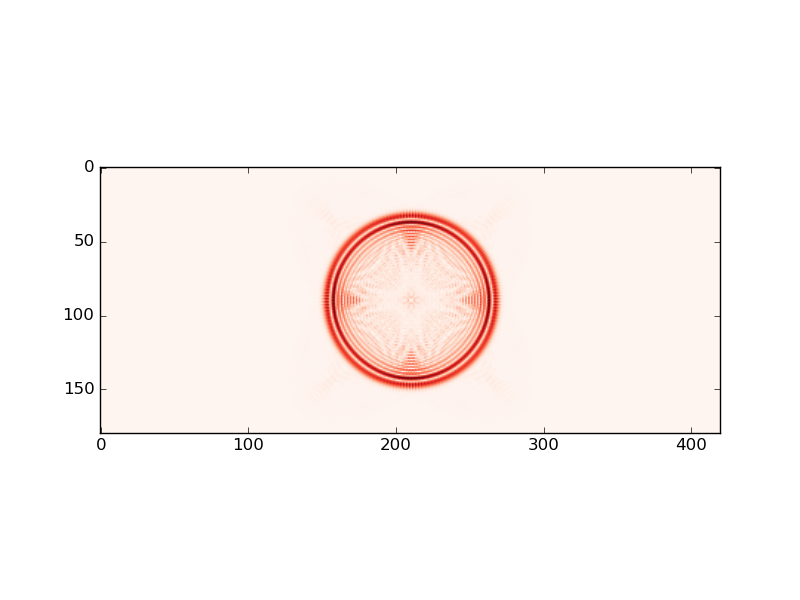
\includegraphics[scale=0.55, trim=45 90 50 90, clip]{images/lbm_simple/lbm_100.png}
		\label{fig:lbm_simple_100}
	}
	\subfigure[300 itérations]{%
	\centering
	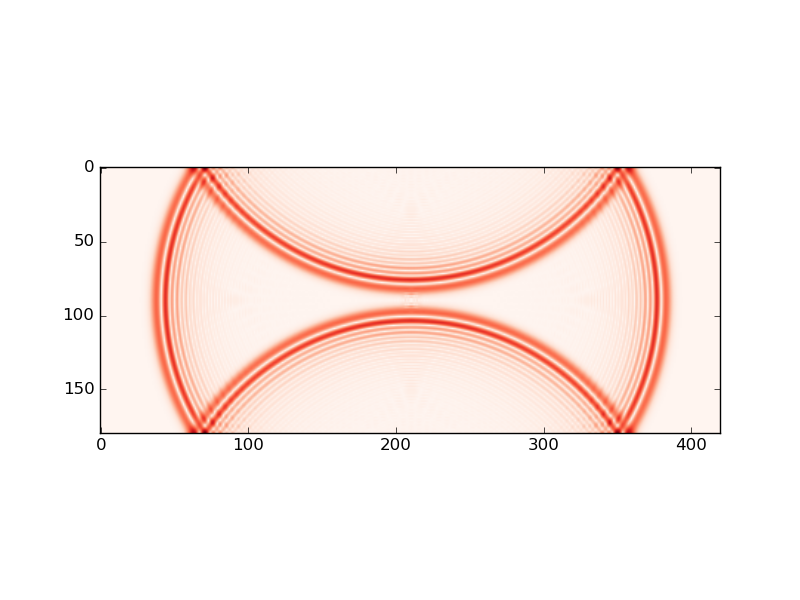
\includegraphics[scale=0.55, trim=45 90 50 90, clip]{images/lbm_simple/lbm_300.png}
	\label{fig:lbm_simple_300}
    }
	\subfigure[500 itérations]{%
		\centering
		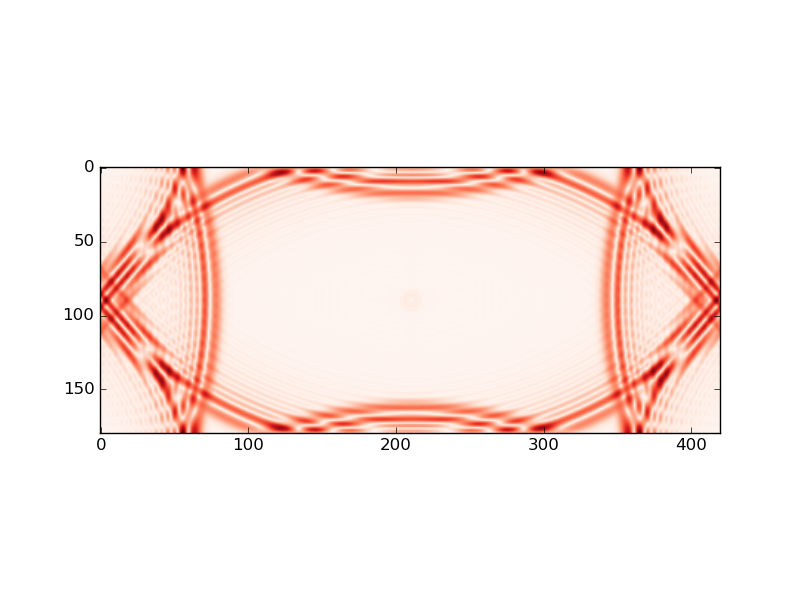
\includegraphics[scale=0.55, trim=45 90 50 90, clip]{images/lbm_simple/lbm_500.png}
		\label{fig:lbm_simple_500}
	}
	\subfigure[1000 itérations]{%
		\centering
		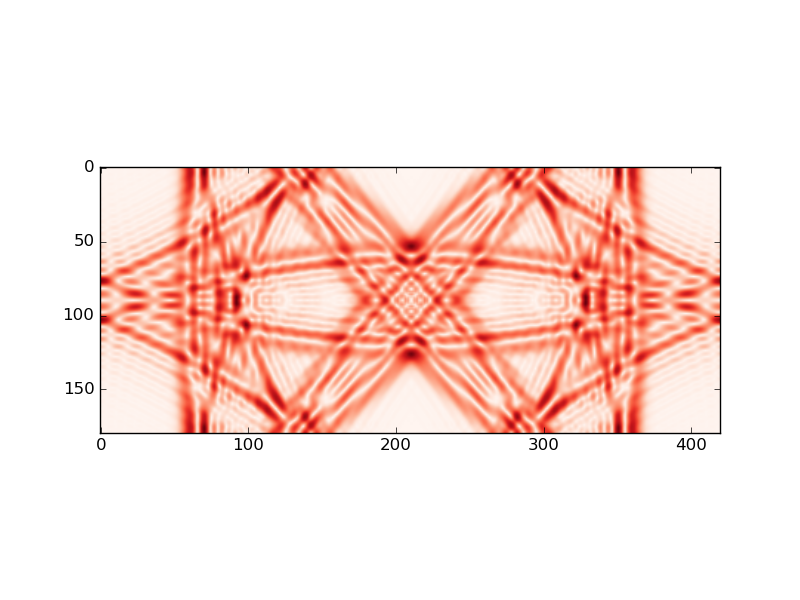
\includegraphics[scale=0.55, trim=45 90 50 90, clip]{images/lbm_simple/lbm_1000.png}
		\label{fig:lbm_simple_1000}
	}
	\caption{Simulation \ac{LBM} simplifiée avec une perturbation au centre du domaine}
	\label{fig:lbm_simple}
\end{figure}

\begin{figure}[h]
	\centering
	\subfigure[20 itérations]{%
		\centering
		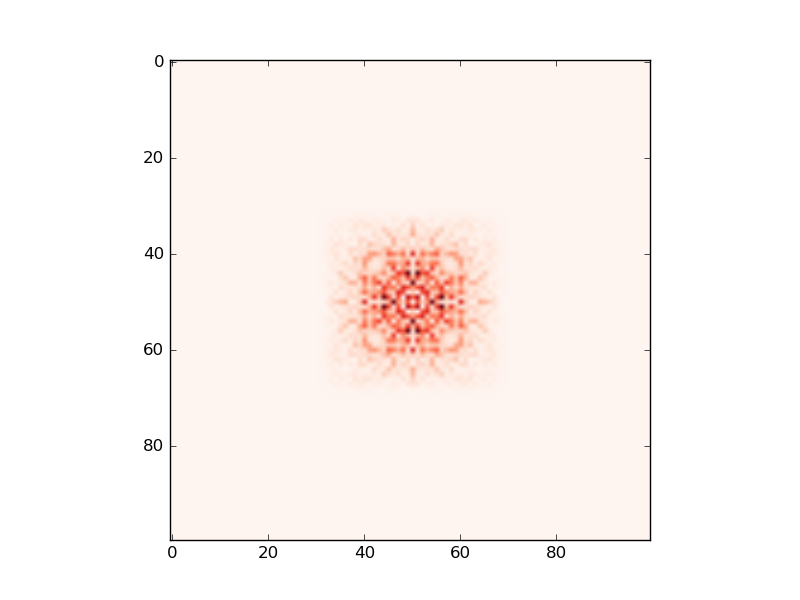
\includegraphics[scale=0.37, trim=103 20 105 40, clip]{images/lbm_simple_3d/lbm_20.png}
		\label{fig:lbm_simple_3d_20}
	}
	\subfigure[60 itérations]{%
		\centering
		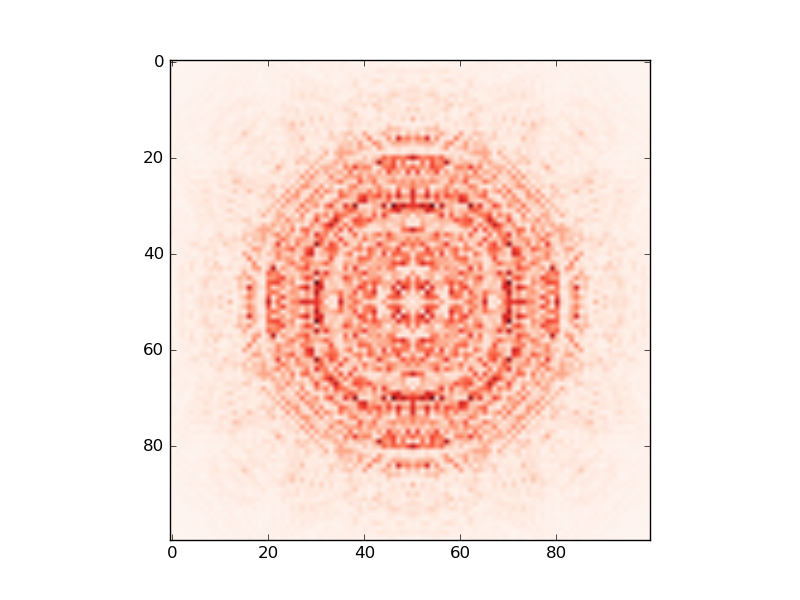
\includegraphics[scale=0.37, trim=103 20 105 40, clip]{images/lbm_simple_3d/lbm_60.png}
		\label{fig:lbm_simple_3d_60}
	}
	\subfigure[100 itérations]{%
		\centering
		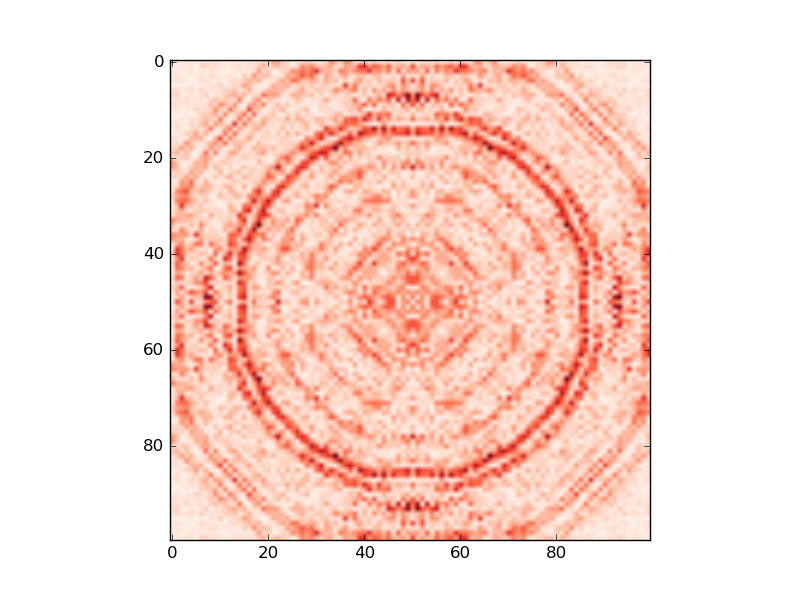
\includegraphics[scale=0.37, trim=103 20 105 40, clip]{images/lbm_simple_3d/lbm_100.png}
		\label{fig:lbm_simple_3d_100}
	}
	\subfigure[140 itérations]{%
		\centering
		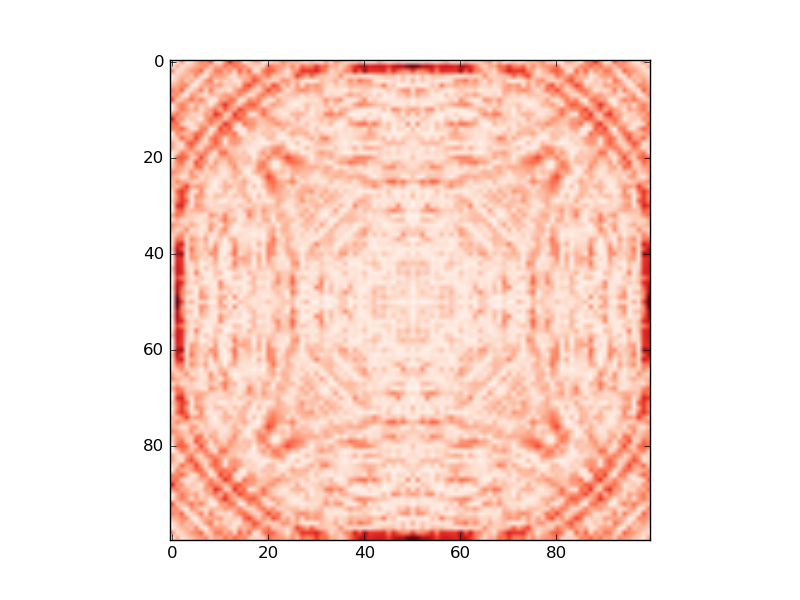
\includegraphics[scale=0.37, trim=103 20 105 40, clip]{images/lbm_simple_3d/lbm_140.png}
		\label{fig:lbm_simple_3d_140}
	}
	\subfigure[180 itérations]{%
		\centering
		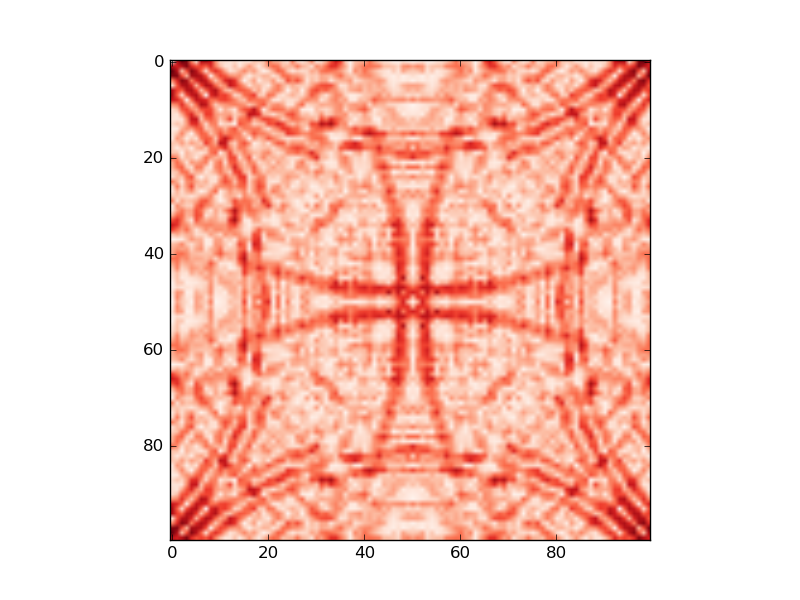
\includegraphics[scale=0.37, trim=103 20 105 40, clip]{images/lbm_simple_3d/lbm_180.png}
		\label{fig:lbm_simple_3d_180}
	}
	\subfigure[220 itérations]{%
		\centering
		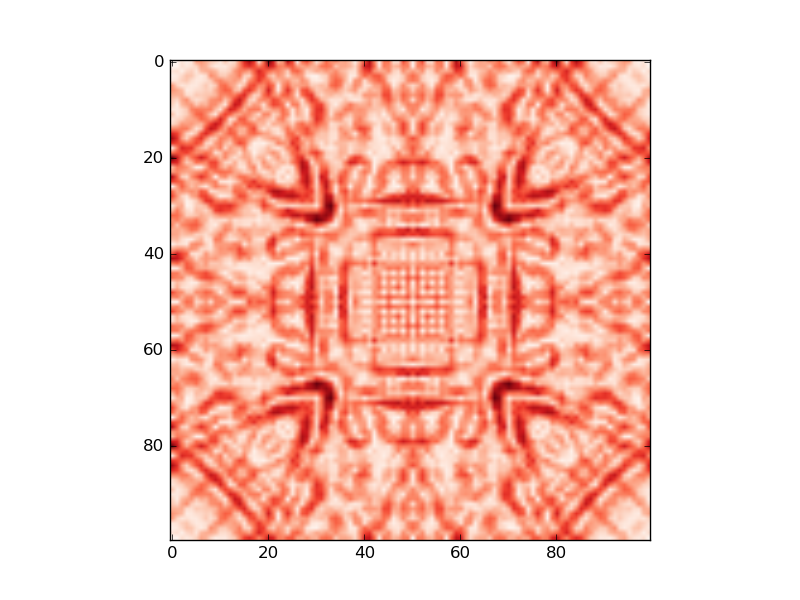
\includegraphics[scale=0.37, trim=103 20 105 40, clip]{images/lbm_simple_3d/lbm_220.png}
		\label{fig:lbm_simple_3d_220}
	}
	\subfigure[260 itérations]{%
		\centering
		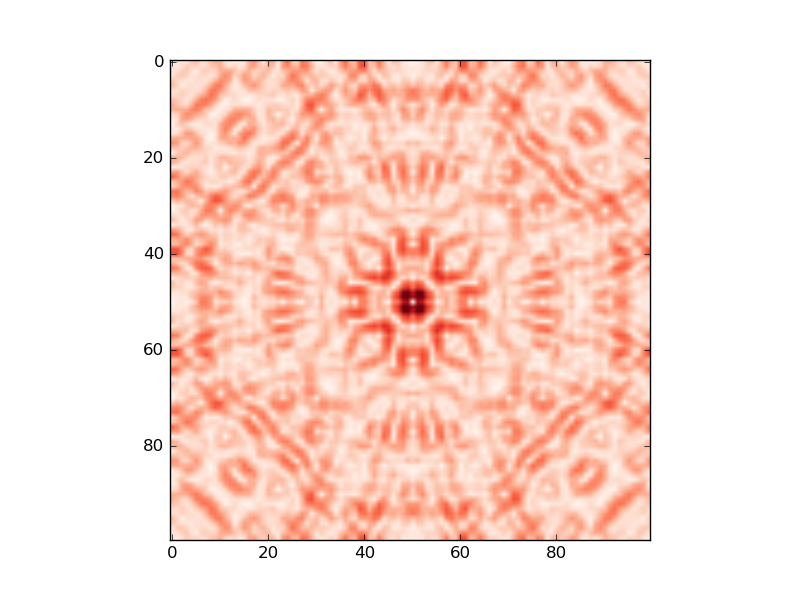
\includegraphics[scale=0.37, trim=103 20 105 40, clip]{images/lbm_simple_3d/lbm_260.png}
		\label{fig:lbm_simple_3d_260}
	}
	\subfigure[300 itérations]{%
		\centering
		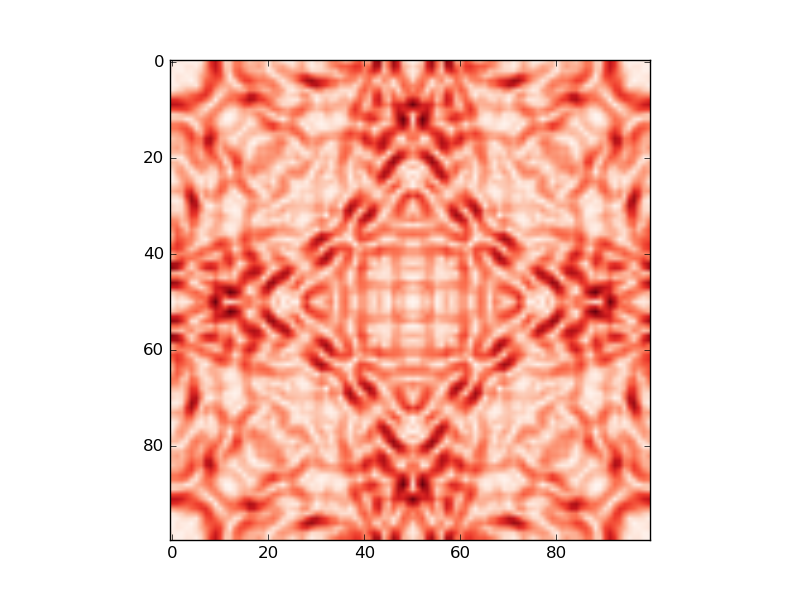
\includegraphics[scale=0.37, trim=103 20 105 40, clip]{images/lbm_simple_3d/lbm_300.png}
		\label{fig:lbm_simple_3d_300}
	}
	\subfigure[340 itérations]{%
		\centering
		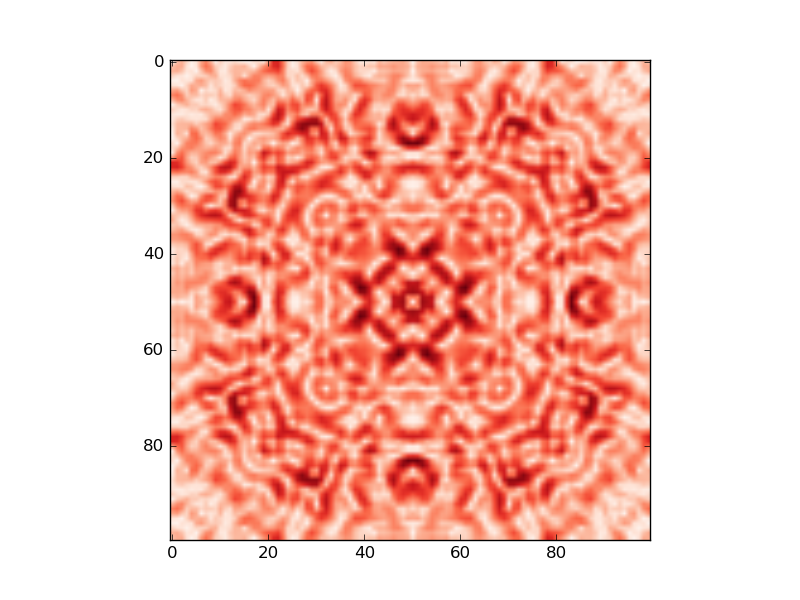
\includegraphics[scale=0.37, trim=103 20 105 40, clip]{images/lbm_simple_3d/lbm_340.png}
		\label{fig:lbm_simple_3d_340}
	}
	\subfigure[380 itérations]{%
		\centering
		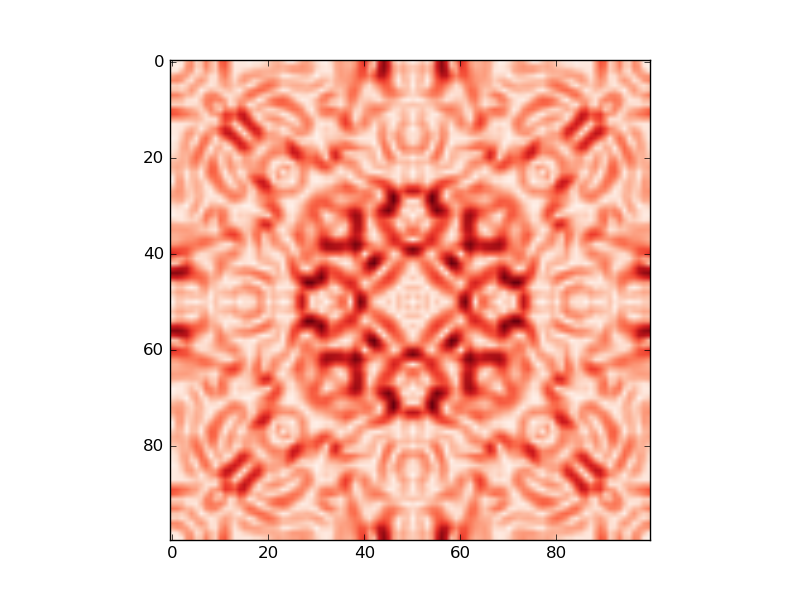
\includegraphics[scale=0.37, trim=103 20 105 40, clip]{images/lbm_simple_3d/lbm_380.png}
		\label{fig:lbm_simple_3d_380}
	}
	\subfigure[420 itérations]{%
		\centering
		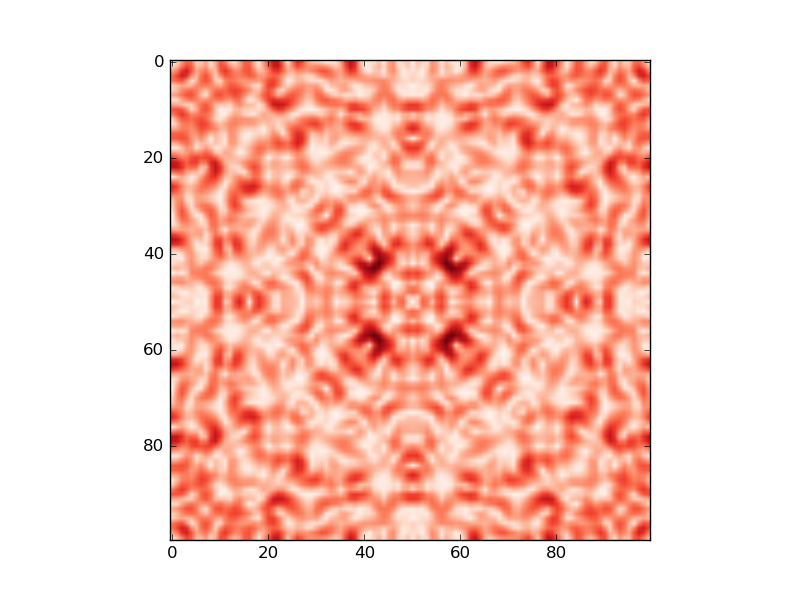
\includegraphics[scale=0.37, trim=103 20 105 40, clip]{images/lbm_simple_3d/lbm_420.png}
		\label{fig:lbm_simple_3d_420}
	}	
	\subfigure[460 itérations]{%
		\centering
		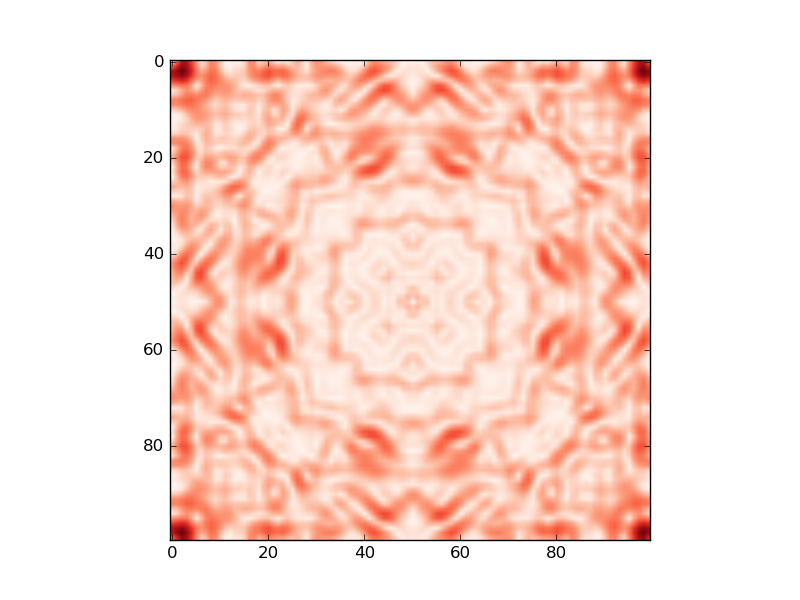
\includegraphics[scale=0.37, trim=103 20 105 40, clip]{images/lbm_simple_3d/lbm_460.png}
		\label{fig:lbm_simple_3d_460}
	}
	\caption{Coupe au centre d'une simulation \ac{LBM} simplifiée en 3D}
	\label{fig:lbm_simple_3d}
\end{figure}

\section{Implémentations Cuda}
\subsection{Sources Cuda de Sailfish}
%\subsubsection{Sources Python et extraction du code Cuda}
Sailfish est un outil de simulation de dynamiques des fluides basés sur la \ac{LBM}. Bien qu'il soit écrit en Python, Sailfish génère, compile et exécute un code Cuda pour optimiser l'exécution de ses simulations sur \acs{GPU}.

Dans leur article, \citet{januszewski_sailfish:_2014} décrivent son fonctionnement général, mais afin d'avoir un aperçu plus concret, une analyse du code est nécessaire. 

Une brève analyse du code Python permet d'identifier que la fonction \texttt{get\_code} génère le code Cuda. Celle-ci est appelée dans le corps de la fonction \texttt{\_update\_compute\_code} du fichier \texttt{sailfish/subdomain\_runner.py} du projet, qui compile ensuite le code généré. À l'aide d'un \acs{IDE} comme PyCharm et d'un point d'arrêt, il est alors possible d'extraire le code Cuda au format \acs{ASCII} avant qu'il soit compilé en langage machine.

Le code Cuda, plus long et plus compliqué qu'escompté, déclare de nombreuses fonctions dont plusieurs semblent avoir une utilité identique. Il est difficile d'identifier quelle portion du code est utilisé, et de quelle façon sans une analyse approfondie du fonctionnement de Sailfish.

\subsection{Code \eg{historique} de Sailfish}
Le projet disponible sur le dépôt Github de Sailfish offre une intéressante implémentation, dans le dossier \texttt{historical}. Ces sources ne font pas partie du reste du projet, mais implémentent de façon simple une simulation D2Q9 de la \acs{LBM} sur \acs{GPU} avec des performances respectables. On y observe les pratiques détaillées ci-dessous.

%\begin{itemize}
%\item \textbf{Utilisation des registres}: 
\subsubsection{Utilisation des registres}
Les populations sont conservées dans la mémoire globale, à disposition de tous les cœurs du \acs{GPU} ainsi que du \acs{CPU} à travers un \texttt{cudaMemcpy}. Toutefois, le temps d'accès à ce type de mémoire est très lent. Plutôt que d'accéder aux populations sur la mémoire globale lors de chaque calcul, celles-ci sont copiées dans des variables locales du kernel. Ces variables, qui se situent dans les registres du \acs{GPU}, le type de mémoire le plus rapide, sont alors utilisées dans les calculs et sont finalement copiées dans la mémoire globale à la fin du kernel.
Cette méthode réduit sensiblement le nombre d'accès à la mémoire globale et augmente ainsi nettement les performances.
%\item \textbf{Structure de donnée des populations}:
\subsubsection{Structure de donnée des populations}
Les populations ne sont pas toutes conservées dans le même tableau en mémoire globale. Chaque direction possède son propre tableau à une dimension.

%\item \textbf{Calcul des populations}: 
\subsubsection{Calcul des populations}
Plutôt qu'utiliser une boucle pour itérer sur les différentes directions et en calculer de façon générique leur état (comme l'equilibrium), celles-ci sont dépliées pour effectuer un à un le calcul adéquat.

%\item \textbf{Streaming sur la mémoire partagée (coalescing)}: 
\subsubsection{\textit{Streaming coalesced}}\label{title-streaming-coalesced}
Le \textit{streaming} copie les directions de la population calculée par un cœur \acs{GPU} dans les populations adjacentes qui résident en mémoire globale. L'accès à cette mémoire est lent, mais peut être optimisé par des accès contigus où l'indice du cœur est aligné à celui du bloc. On dit de ce schéma d'accès à la mémoire qu'il est \eg{\textit{coalesced}}.

Les \textit{threads} au sein d'un bloc sont activés par \textit{warp} de 32\footnote{ce nombre peut dépendre de la génération du \ac{GPU} utilisé} sur l'axe des \textit{x}. Ces \textit{threads}, qui accèdent à la mémoire globale lors du \textit{streaming}, doivent chacun y écrire une à une les valeurs des directions calculées qui résident dans leurs registres, soit 32 doubles par direction. La mémoire globale est accédée par transaction de 32, 64, 128 ou 256 octets. Par conséquent, si les 32 directions (qui occupent 256 octets) accédées par les \textit{threads} sont contiguës en mémoires, seule une transaction en mémoire globale par direction est nécessaire. 

Les figures \ref{fig:sailfish_hist_misaligned}, \ref{fig:sailfish_hist_alignment}, \ref{fig:sailfish_hist_dir_misaligned}, \ref{fig:sailfish_hist_ti}, \ref{fig:sailfish_hist_aligned} et \ref{fig:sailfish_hist_dir_aligned} illustrent le \textit{streaming} d'un bloc de 4 \textit{threads} sur un domaine $12 \times 3$.
Sur la figure \ref{fig:sailfish_hist_misaligned}, les \textit{threads} utilisent un schéma d'accès où les directions sont propagées aux populations adjacentes directement en mémoire globale. L'arrangement en mémoire des directions sur les populations accédées est illustré sur la figure \ref{fig:sailfish_hist_alignment}. On y observe sur la figure~\ref{fig:sailfish_hist_dir_misaligned} que l'écriture des valeurs pour les directions nord et sud est naturellement alignée. Ce n'est toutefois pas le cas pour les autres directions puisqu'elles impliquent un décalage en $y$ (est ou ouest). En effet, l'index des \textit{thread} au sein de leur bloc n'est plus aligné à celui du \textit{thread} du segment accédé par la transaction en mémoire globale. Leur accès n'est par conséquent pas \textit{coalesced}.

\begin{figure}[h]
	\centering
	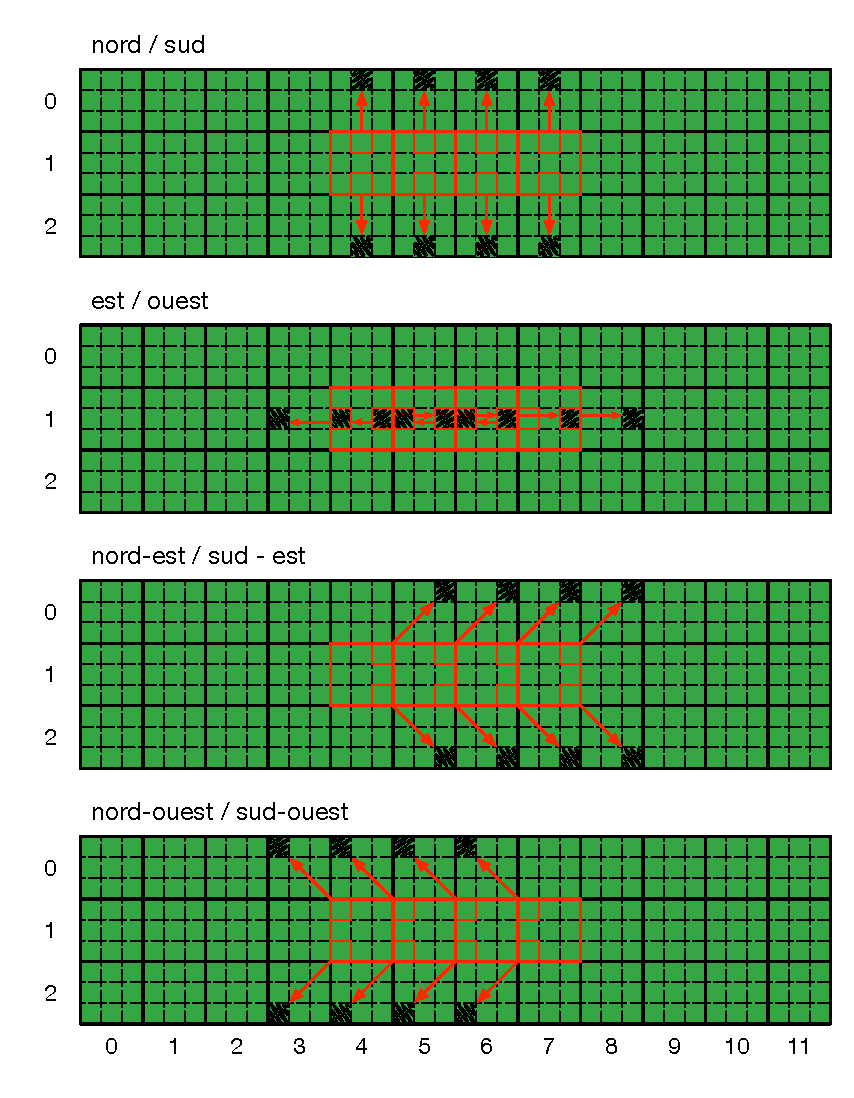
\includegraphics[fbox,scale=1.05]{images/streaming/sailfish_hist_misaligned.pdf}
	\caption{\textit{Streaming} \textit{uncoalesced} d'un bloc de quatre \textit{threads}}
	\label{fig:sailfish_hist_misaligned}
\end{figure}

\begin{figure}[h]
	\centering
	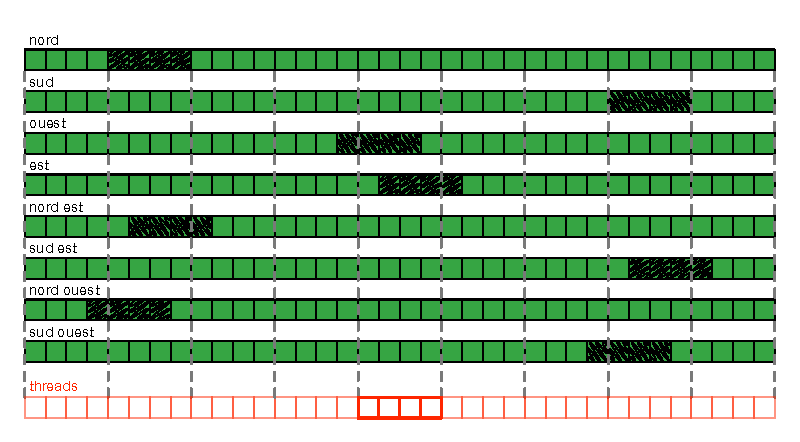
\includegraphics[fbox,scale=1.1]{images/streaming/sailfish_hist_alignment.pdf}
	\caption{Arrangement en mémoire des populations du \textit{streaming} de la figure \ref{fig:sailfish_hist_misaligned}}
	\label{fig:sailfish_hist_alignment}
\end{figure}

Pour remédier au désalignement inhérent à la position population calculée par chaque \textit{thread}, une stratégie en deux étapes est utilisée pour écrire les directions en mémoire globale (figure \ref{fig:sailfish_hist_ti}). 
\begin{enumerate}
\item Dans un premier temps, au lieu de les propager directement en mémoire globale, les directions nord-ouest, ouest et sud-ouest de chaque \textit{thread} au sein d'un bloc sont écrites en mémoire partagée sur l'indice du \textit{thread} de gauche ($x-1$) et les directions nord-est, est et sud-est sur l'indice du \textit{thread} de droite ($x+1$).
\item Dans un second temps, chaque \textit{thread} propage en mémoire globale les directions inscrites à son indice aux populations en dessus ($x - 12$) et en dessous ($x + 12$).
\end{enumerate}
Une barrière de synchronisation entre les deux étapes assure que chaque \textit{thread} ait bien calculé et inscrit les directions en mémoire partagée, à l'attention de ses voisins, avant de procéder à la seconde étape.

Les directions nord et sud, étant par nature alignées, sont directement propagées en mémoire globale, indépendamment lors de la première ou seconde étape\footnote{illustré ici lors de la première étape de la figure \ref{fig:sailfish_hist_aligned}}. 

La figure \ref{fig:sailfish_hist_aligned} illustre ce mécanisme exécuté simultanément sur chaque \textit{thread} d'un bloc et \ref{fig:sailfish_hist_dir_aligned} l'alignement des indices des accès en mémoire globale. On constate avec cette stratégie des accès \textit{coalesced}, à l'exception de ceux des \textit{thread} au bord du bloc. En effet, ces derniers n'ont pas accès à la mémoire partagée du \textit{thread} adjacent qui se trouve dans un bloc différent. Ils doivent par conséquent propager certaines directions directement en mémoire globale.

L'exemple utilisé illustre des blocs de 4 \textit{thread} par souci de lisibilité, mais dans la pratique, des blocs plus grands (32 ou 64) sont utilisés pour réduire ainsi le nombre d'accès \textit{uncoalesced}.

Toutefois, \citet{obrecht_global_2011} cherchent à éviter l'usage de la mémoire partagée plutôt qu'éviter à tout prix les accès \textit{uncoalesced}. En effet, cette stratégie se montre efficace sur les anciennes générations de \acs{GPU}, le gain en performance semble nettement moindre sur les \acs{GPU} récents, qui réduisent le coût des accès \textit{uncoalesced} à l'aide de la mémoire cache. 
%\end{itemize}


\begin{figure}[h]
	\centering
	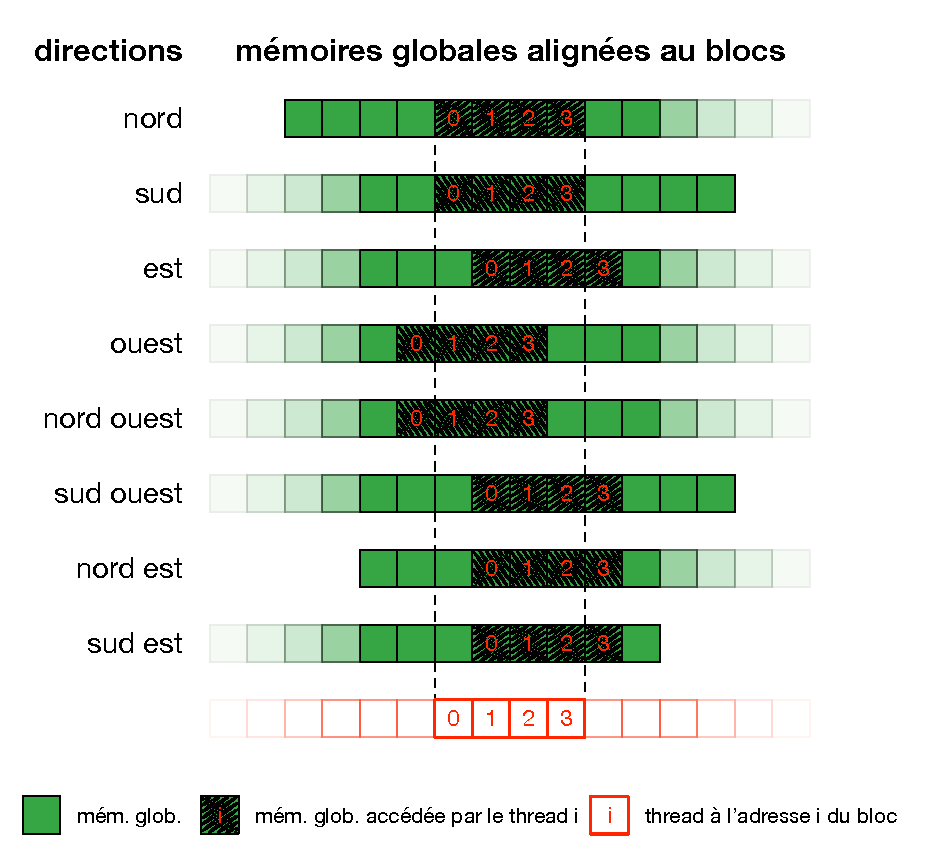
\includegraphics[fbox,scale=0.95]{images/streaming/sailfish_hist_dir_misaligned.pdf}
	\caption{Accès mémoire désaligné des \textit{threads} lors du \textit{streaming} de la figure \ref{fig:sailfish_hist_misaligned}}
	\label{fig:sailfish_hist_dir_misaligned}
\end{figure}

\begin{figure}[h]
	\centering
	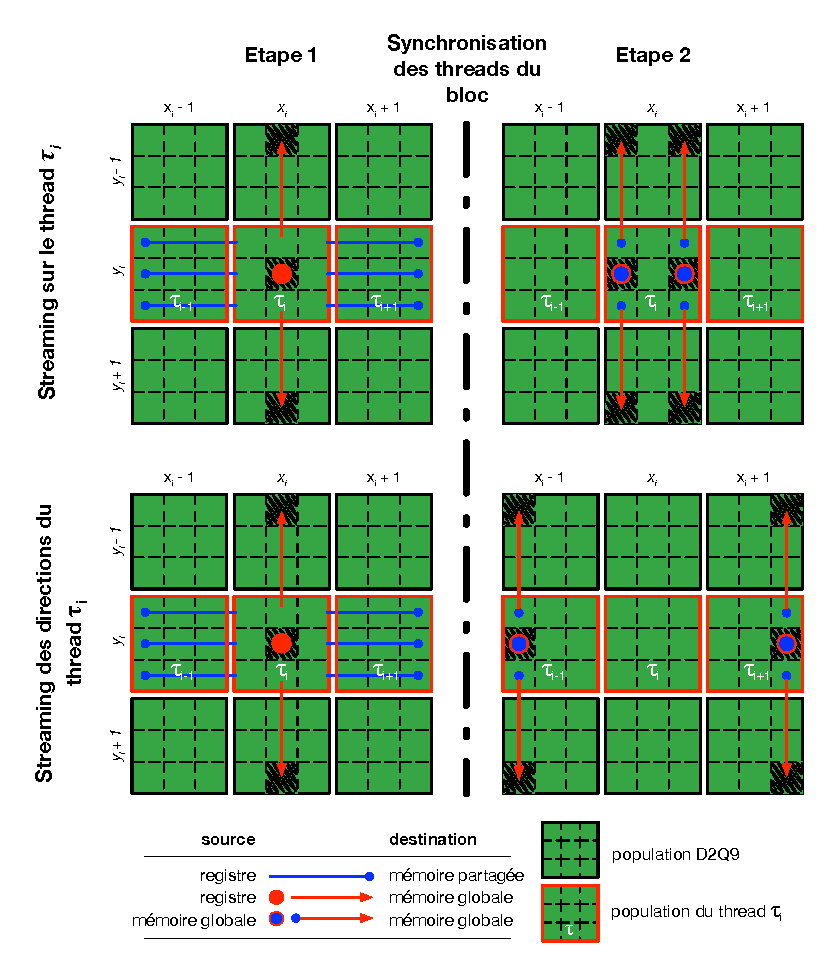
\includegraphics[fbox,scale=1.1]{images/streaming/sailfish_hist_ti.pdf}
	\caption{Stratégie de \textit{streaming} \textit{coalesced} par réalignement des populations en mémoire partagée}
	\label{fig:sailfish_hist_ti}
\end{figure}


\begin{figure}[h]
	\centering
	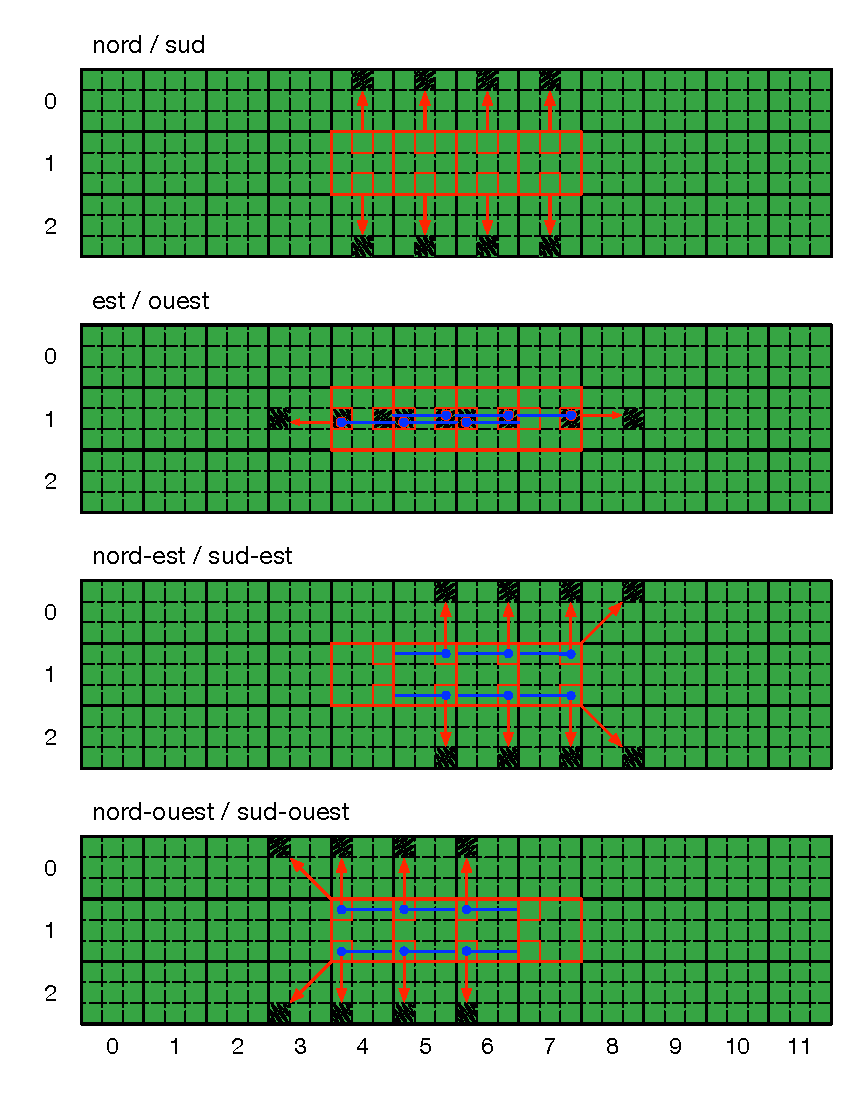
\includegraphics[fbox,scale=1.05]{images/streaming/sailfish_hist_aligned.pdf}
	\caption{\textit{Streaming} \textit{coalesced} d'un bloc de quatre \textit{threads}}
	\label{fig:sailfish_hist_aligned}
\end{figure}

\begin{figure}[h]
	\centering
	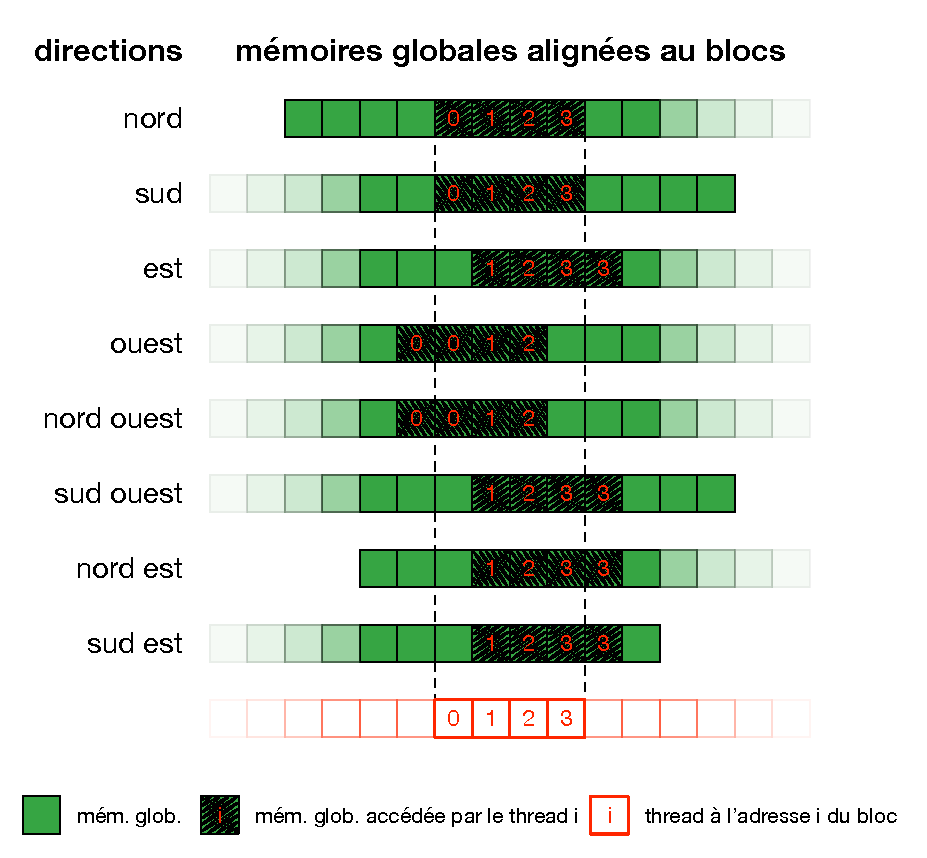
\includegraphics[fbox,scale=0.95]{images/streaming/sailfish_hist_dir_aligned.pdf}
	\caption{Accès mémoire aligné des \textit{threads} lors du \textit{streaming} de la figure \ref{fig:sailfish_hist_aligned}}
	\label{fig:sailfish_hist_dir_aligned}
\end{figure}

\subsection{Différences entre calculs sur CPU et GPU} \label{title-floats}
Cuda supporte la norme IEEE 754 pour les calculs avec nombre flottants \cite{noauthor_cuda_2017}. Toutefois, dans la première implémentation Cuda de la \acs{LBM}, le protocole de test (décrit en section \ref{title-tests}) a montré des différences sur certains calculs réalisés par les codes \ac{CPU}.

Pour les mesurer, un code \ac{LBM} 2D \ac{CPU} et un code \ac{GPU} ont été implémentés et leurs résultats comparés. La figure \ref{fig:lbm_float_deltas} illustre la différence moyenne entre les valeurs calculées sur \ac{CPU} et \ac{GPU} pour l'ensemble des populations $f_{in}$ de chaque itération.

\begin{figure}[H]
	\centering
	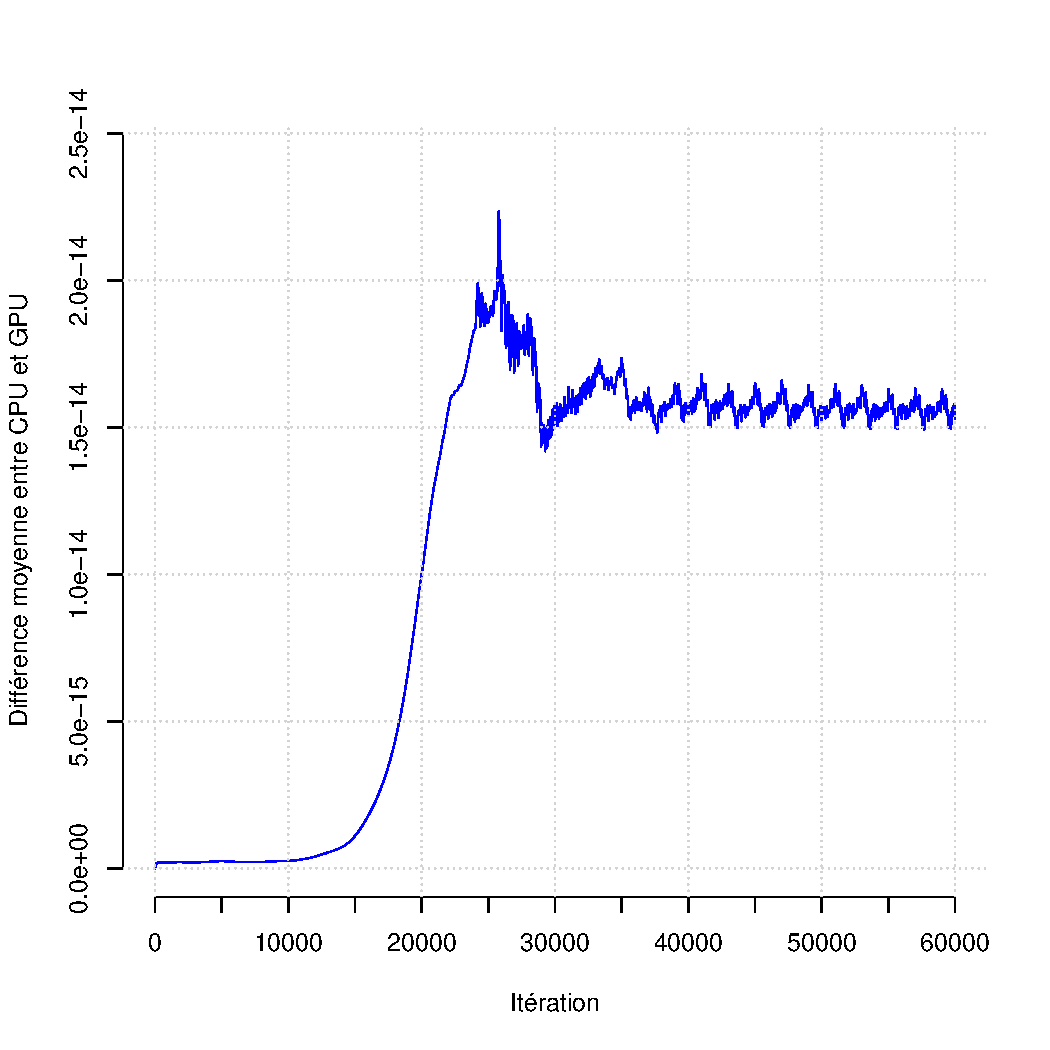
\includegraphics[scale=0.87, fbox]{../data/lbm_cpu_vs_gpu/deltas/Rplots.pdf}
	\caption{Différences moyennes (par itération) entre les calculs sur \acs{CPU} et \acs{GPU}}
	\label{fig:lbm_float_deltas}
\end{figure}

L'écart entre les résultats observés sur \ac{CPU} et \ac{GPU} suit les étapes de la simulation réalisée (fluide autour d'un cylindre) illustrée par les figures \ref{fig:lbm_5000_to_43000}:
\begin{itemize}
	\item entre 0 et environ 12000 itérations, une trace se forme derrière le cylindre et l'écart moyen reste faible et stable (quinze zéros après la virgule);
	\item entre 15000 et 20000 itérations, la trace commence à osciller et l'écart augmente brutalement (treize zéros après la virgule);
	\item à la 25792$^{\textrm{ième}}$ itération, l'oscillation commence à se stabiliser et l'écart atteint son maximum (toujours treize chiffres après la virgule);
	\item dès environ 36000 itérations, l'oscillation est stabilisée (comme le montrent les figures \ref{fig:lbm_39000} et \ref{fig:lbm_43000}, le même motif réapparaît toutes les 4000 itérations environ) et les écarts avec.
\end{itemize}

\begin{figure}[h]
	\centering
	\subfigure[5000 itérations]{%
		\centering
		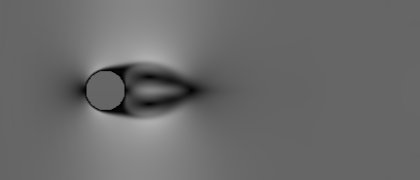
\includegraphics[scale=0.5]{../data/lbm_images/cpu_lbm_5000.png}
		\label{fig:lbm_5000}
	}
	\subfigure[10000 itérations]{%
		\centering
		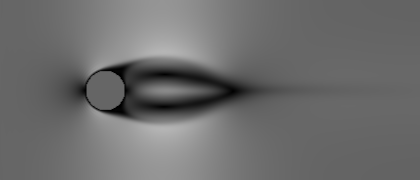
\includegraphics[scale=0.5]{../data/lbm_images/cpu_lbm_10000.png}
		\label{fig:lbm_10000}
	}
	\subfigure[15000 itérations]{%
		\centering
		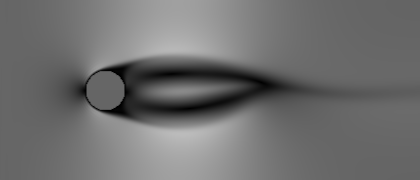
\includegraphics[scale=0.5]{../data/lbm_images/cpu_lbm_15000.png}
		\label{fig:lbm_15000}
	}
	\subfigure[20000 itérations]{%
		\centering
		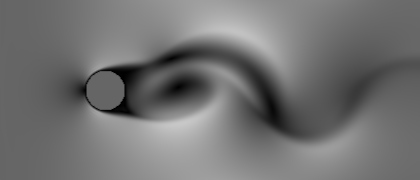
\includegraphics[scale=0.5]{../data/lbm_images/cpu_lbm_20000.png}
		\label{fig:lbm_20000}
	}
	\subfigure[25792 itérations]{%
		\centering
		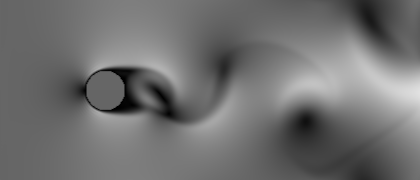
\includegraphics[scale=0.5]{../data/lbm_images/cpu_lbm_25792.png}
		\label{fig:lbm_25792}
	}
	\subfigure[39000 itérations]{%
		\centering
		\includegraphics[scale=0.5]{../data/lbm_images/cpu_lbm_39000.png}
		\label{fig:lbm_39000}
	}
	\subfigure[40000 itérations]{%
		\centering
		\includegraphics[scale=0.5]{../data/lbm_images/cpu_lbm_40000.png}
		\label{fig:lbm_40000}
	}
	\subfigure[41000 itérations]{%
		\centering
		\includegraphics[scale=0.5]{../data/lbm_images/cpu_lbm_41000.png}
		\label{fig:lbm_41000}
	}
	\subfigure[42000 itérations]{%
		\centering
		\includegraphics[scale=0.5]{../data/lbm_images/cpu_lbm_42000.png}
		\label{fig:lbm_42000}
	}
	\subfigure[43000 itérations]{%
		\centering
		\includegraphics[scale=0.5]{../data/lbm_images/cpu_lbm_43000.png}
		\label{fig:lbm_43000}
	}
	\caption{Simulation \ac{LBM} d'un fluide autour d'un cylindre}
	\label{fig:lbm_5000_to_43000}
\end{figure}

Cette différence entre certains résultats sur \ac{CPU} et \ac{GPU} est le fruit d'une optimisation du compilateur Cuda. Sur \ac{CPU}, lorsqu'une opération du type $r = x \times y+z$ est rencontrée, le processeur calcul d'abord $r_{xy} = x \times y$ puis $r = r_{xy} + z$. Deux opérations sont donc réalisées, ce qui implique deux potentiels arrondis dans le cas des nombres flottants. Sur \ac{GPU}, le compilateur optimise ce type de calculs \cite{noauthor_cuda_2017-1} avec la fonction \ac{FMA} qui réalise $x \times y+z$ en une seule opération. Le calcul est ainsi plus rapide et précis (puisqu'un seul arrondi est effectué).

Comme le souligne la documentation de Cuda, cette optimisation n'est pas forcément souhaitable dans certaines circonstances et peut être évitée avec l'utilisation de fonctions intrinsèques \cite{noauthor_cuda_2017-1, noauthor_cuda_2017-2}.

Cette précaution force le \ac{GPU} à effectuer les multiplications et additions indépendamment et permet de s’assurer que les calculs réalisés sur \ac{CPU} et \ac{GPU} produisent les mêmes résultats.

\subsection{Passage de la 2D à la 3D et bibliothèque \texttt{lbmcuda}}
De nombreuses implémentations 2D ont été réalisées. Elles ont d’abord été adaptées des portages en C, puis inspirées par le code historique de Sailfish, jusqu’à la dernière (nommé \texttt{lbm\_opt2}) qui a fini par atteindre des performances acceptables (450 MLUPS sur une Nvidia GeForce GT 750M). 

Les 10 populations manquantes sont ajoutées en mémoire globale, aux divers calculs nécessaires à leur simulation ainsi qu'au \textit{streaming}. À ce stade, l'implémentation utilisait encore la mémoire partagée pour le \textit{streaming}. Suite à l'ajout des populations, l'implémentation est testée avec et sans ce mécanisme. Mais comme l'évoque la section \ref{title-streaming-coalesced}, il s'avère que les \textit{GPU} récents ne pâtissent pas réellement des accès \textit{uncoalesced} en raison d'optimisation automatique à travers l'utilisation de la mémoire cache.

D'autres optimisations, proposées par \citet{januszewski_sailfish:_2014} et \citet{tran_performance_2017} améliorent les performances:
\begin{itemize}
\item \textbf{Registres}: Les registres sont utilisés par certaines variables locales du kernel. C'est le type de mémoire le plus rapide, mais leur nombre est restreint. En dépasser la limite entraîne un débordement en mémoire local, moins rapide, et par conséquent une perte de performance. Hélas, le passage de D2Q9 à D3Q19 augmente significativement le nombre de variables locales et par conséquent l'utilisation des registres. Ne pas précalculer des valeurs utilisées plusieurs fois, et qui devraient être ainsi stockées dans des variables intermédiaires, mais les recalculer à chaque fois semble être une \eg{optimisation} contre-intuitive, mais réduit le nombre de registres et par conséquent contribue à améliorer les performances.
\item \textbf{Cache L1}: \citet{januszewski_sailfish:_2014} relèvent que les accès à la mémoire locale dus aux dépassements du nombre de registres passent par la cache L1 et que plus sa part inutilisée est grande et moins la mémoire globale est mise à contribution. Ils proposent ainsi d'augmenter la taille de la cache et de désactiver la cache L1 pour les accès à la mémoire globale. La première opération est accomplie par \texttt{cudaDeviceSetCacheConfig}:
\begin{lstlisting}[numbers=none]
if ( cudaDeviceSetCacheConfig (cudaFuncCachePreferL1) != cudaSuccess)
	fprintf(stderr, "cudaFuncSetCacheConfig failed\n");
\end{lstlisting}
et la seconde en compilant le code Cuda avec les arguments \texttt{-Xptxas -dlcm=cg}.
\item \textbf{Divisions par des multiplications}: Les multiplications sont un peu plus rapides que les divisions. Remplacer une division par une multiplication, lorsque cela est possible, peut ainsi améliorer les performances. Si plusieurs calculs requièrent une division par la même valeur (comme avec \textit{rho} dans la fonction \textit{macroscopic}), l'inverse de sa valeur peut être calculé initialement puis être multiplié par la suite pour éviter plusieurs divisions. Cette méthode a toutefois l'inconvénient de modifier parfois très légèrement le résultat du calcul en raison d'un arrondi différent avec les valeurs flottantes et ajoute une variable locale intermédiaire.
\end{itemize}

Finalement, en vue de son intégration à Palabos et afin d'en simplifier l'utilisation, l'implémentation Cuda est portée dans une bibliothèque dynamique nommée \texttt{lbmcuda} que le projet \texttt{lbm\_simple\_lbmcuda} utilise pour implémenter la même configuration que \texttt{lbm\_simple} en C et Python. La bibliothèque implémente les principales fonctions suivantes:

\begin{itemize}
\item \texttt{lbm\_simulation\_create}: Créer un domaine de simulation en spécifiant ses dimensions ainsi que la valeur d'omega.
\item \texttt{lbm\_simulation\_update}: Mets à jour les populations de domaine sur une itération.
\item \texttt{lbm\_lattices\_read} et \texttt{lbm\_lattices\_read}: Transfert l'intégralité des populations du domaine respectivement depuis et vers le \acs{GPU}.
\item \texttt{lbm\_lattices\_read\_subdomain} et \texttt{lbm\_lattices\_write\_subdomain}: Transfert partiel du domaine.
\item \texttt{lbm\_read\_palabos\_subdomain} et \texttt{lbm\_write\_palabos\_subdomain} : Transfert partiel du domaine avec réorganisation mémoire selon l'ordre utilisé par Palabos (voir section \ref{title-strategie_reorganisation}).
\end{itemize}

\section{Intégration à Palabos}
\subsection{Co-processeurs}
\subsubsection{Fonctionnement}
Il est possible de demander à Palabos de découper un domaine de recherche en plusieurs sous-domaines afin de les calculer indépendamment les uns des autres. Comme l'illustre la figure \ref{fig:plb_domain_split}, un sous-domaine possède une portion unique du domaine de recherche (vert) ainsi qu'une marge extérieure (bleu) qui s'entrelace avec les zones centrales des sous-domaines adjacents. Son rôle est de propager les valeurs calculées par les sous-domaines voisins pour calculer la zone centrale (verte).

\begin{figure}[h]
	\centering
	\includegraphics[scale=0.65, fbox]{images/decoupage_domaine_palabos.pdf}
	\caption{Découpage d'un domaine 12x4 en trois sous-domaines par Palabos}
	\label{fig:plb_domain_split}
\end{figure}

Ce découpage permet
\begin{enumerate*}
\item de distribuer la simulation sur différents nœuds (à l'aide d'\acs{MPI}) et
\item de déléguer les calculs à un \ac{CP} spécialisé.
\end{enumerate*}

Un \ac{CP} (ou accélérateur) est un module capable de calculer l'état d'un sous-domaine, normalement pris en charge par Palabos sur \ac{CPU}, mais cette fois confié par celui-ci. Son objectif est d'accélérer la vitesse des calculs en se spécialisant sur un certain type de sous-domaine. L'utilisation d'un \ac{CP} est illustrée dans le programme d'exemple \texttt{coProcessor}\footnote{dossier: \texttt{<palabos root>/examples/codesByTopic/coProcessor}} fourni dans Palabos où l'on distingue cinq étapes importantes.

\begin{enumerate}
\item \textbf{Initialisation des \ac{CP}}: On commence par assigner un \ac{CP} aux sous-domaines désignés d'un espace de recherche découpé au préalable.
\item \textbf{Transfert \ac{CPU} à \ac{CP}}: À ce stade, seul Palabos connaît l'état de l'espace de recherche. Par conséquent, on transfère les valeurs des populations dans les sous-domaines délégués aux \ac{CP}.
\item \textbf{Calcul du \ac{CS}}: On calcule \textit{une} itération avec la \ac{LBM} sur l'ensemble des sous-domaines (avec Palabos et les \ac{CP}).
\item \textbf{Transfert \ac{CP} à \ac{CPU}}: À ce stade, contrairement à la seconde étape, Palabos ignore l'état des sous-domaines assignés au \ac{CP}, que seuls eux connaissent. On transfère cette fois ces valeurs dans le sens opposé.
\item \textbf{Duplication des chevauchements}:  Les enveloppes des sous-domaines se chevauchent. Il faut par conséquent dupliquer les valeurs d'un sous-domaine, calculé à l'étape précédente, dans les enveloppes des sous-domaines voisins.
\end{enumerate}

Au terme de ce processus, une itération complète est ainsi effectuée. Pour en calculer une autre, on recommencera depuis la seconde étape. 

\subsubsection{Implémentation}
Un co-processeur n'est autre qu'une classe qui hérite de \texttt{CoProcessor3D}. Pour fonctionner, elle doit implémenter les principales méthodes suivantes. Elles sont respectivement appelées lors des quatre premières étapes mentionnées précédemment.

\begin{itemize}
\item \texttt{addDomain}: Associe un \texttt{ID} à un sous-domaine attribué au \ac{CP} et en défini les dimensions.
\item \texttt{send}: Envoie l'état du sous-domaine, de la mémoire de Palabos vers celle du \ac{CP}.
\item \texttt{collideAndStream}: Calcul une itération avec la \ac{LBM} sur un sous-domaine du \ac{CP}.
\item \texttt{receive}: Envoie l'état du sous-domaine, de la mémoire du \ac{CP} vers celle de Palabos.
\end{itemize}

C'est ce mécanisme de \ac{CP} qui est utilisé pour donner à Palabos la capacité de calculer sur \acs{GPU}.

\subsection{Transfert mémoire entre Palabos et un \acs{CP} }\label{title-transfert_palabos_cp}
À chaque itération, il est nécessaire de transférer l'état des populations des sous-domaines deux fois:
\begin{enumerate}
\item \textbf{Avant de calculer les populations des \ac{CP}}: depuis Palabos vers les \ac{CP}, pour propager les populations calculées par les sous-domaines adjacents.
\item \textbf{Après les avoir calculés sur les \ac{CP}}: depuis les \ac{CP} vers Palabos, pour propager leurs populations à l'itération suivante.
\end{enumerate}

Lors de l'appel à méthode \textit{send} et \textit{receive}, Palabos transmet un espace mémoire contiguë où les populations sont respectivement écrites et lues. Il est adressé en calculant l'index suivant:
\begin{equation}
i_{pal} = ( x*N_z*N_y + y*N_z + z) * 19 + dir
\end{equation}
avec la dimension  $N_y$ et $N_z$ du sous-domaine en $y$ et $z$ et $i_{pal}$ l'index de la population en $\{x,y,z\}$ avec pour direction $dir$ (figure \ref{fig:plb_population_index}):

\noindent\begin{minipage}{.25\linewidth}
\begin{align*}
&dir_{center} &=  0 \\
&dir_{west} &=  1 \\
&dir_{south} &=  2 \\
&dir_{center}^{bottom} &=  3 \\
&dir_{south west} &=  4
\end{align*}
\end{minipage}%
\begin{minipage}{.25\linewidth}
\begin{align*}
&dir_{north west} &=  5 \\
&dir_{west}^{bottom} &=  6 \\
&dir_{west}^{top} &=  7 \\
&dir_{south}^{bottom} &=  8 \\
&dir_{south}^{top} &=  9 
\end{align*}
\end{minipage}%
\begin{minipage}{.25\linewidth}
\begin{align*}
&dir_{east} &= 10 \\
&dir_{north} &= 11 \\
&dir_{center}^{top} &= 12 \\
&dir_{north east} &= 13 \\
&dir_{south east} &= 14 
\end{align*}
\end{minipage}
\begin{minipage}{.25\linewidth}
\begin{align*}
&dir_{east}^{top} &= 15 \\
&dir_{east}^{bottom} &= 16 \\
&dir_{north}^{top} &= 17 \\
&dir_{north}^{bottom} &= 18\\
\end{align*}
\end{minipage}\\

Si le \ac{CP} utilise la même stratégie d'adressage, une simple copie de la mémoire suffit. Dans le cas inverse, il faut considérer une étape de réorganisation de la mémoire.

\begin{figure}[h]
	\centering
	\includegraphics[scale=0.85, fbox]{images/index_population_palabos.pdf}
	\caption{Adressage d'une population sur Palabos}
	\label{fig:plb_population_index}
\end{figure}

La communication des données entre le \acs{CPU} et le \acs{GPU} passe par la mémoire globale du \acs{GPU} à l'aide de la fonction \texttt{cudaMemcpy}. Ce type de transactions doit être réduit au minimum (au début d'une simulation à des fins d'initialisation et à la fin pour rapatrier les résultats en général) car il s'agit du type d'accès mémoire le plus lent dans le contexte des \acs{GPU}. Hélas, Palabos requiert impérativement ces transactions à chaque itération, ce qui réduit significativement les performances.

Toutefois, il n'est pas nécessaire de transférer l'intégralité du sous-domaine à son \ac{CP} à chaque fois, à l'exception des cas suivants:
\begin{enumerate}
\item lors de la première itération, où il faut initialiser le sous-domaine avec les populations initiales depuis Palabos;
\item après une itération où l'on désire connaître l'état du domaine de recherche, où il faut rapatrier le sous-domaine.
\end{enumerate}

En effet, comme l'illustre la figure \ref{fig:plb_enveloppes}, seules les communications de l'enveloppe extérieure et intérieure sont nécessaires.
L'enveloppe extérieure lors de l'envoi (de Palabos au \ac{CP}), pour permettre la propagation vers l'intérieur du sous-domaine lors du \ac{CS} et l'enveloppe intérieure lors de la réception (du \ac{CP} vers Palabos) pour mettre à jour les enveloppes extérieures des sous-domaines adjacents lors de la duplication des chevauchements (\textit{Duplicate overlaps}) en préparation de l'itération suivante. 

\begin{figure}[h]
	\centering
	\includegraphics[scale=0.62, fbox]{images/enveloppes_interrieures_exeterrieures.pdf}
	\caption{Enveloppe extérieure et intérieure}
	\label{fig:plb_enveloppes}
\end{figure}

Un mécanisme est prévu par Palabos pour ne demander que le transfert de cette enveloppe. Lorsqu'il est utilisé, Palabos procède à un appel à \texttt{send} ou \texttt{receive} par face de l'enveloppe (figure \ref{fig:plb_enveloppe_3d}), soit six appels. Bien que cela représente une multiplication par 6 du nombre d'appels (et par conséquent de l'overhead lié aux \texttt{cudaMemcpy}), cette méthode permet de réduire significativement l'espace mémoire à copier (figure \ref{fig:plb_full_vs_partial_transfert}).

\begin{figure}[h]
	\centering
	\includegraphics[scale=0.75, fbox]{images/enveloppe_3d_palabos.pdf}
	\caption{Enveloppe Palabos 3D}
	\label{fig:plb_enveloppe_3d}
\end{figure}

\begin{figure}[h]
	\centering
	\includegraphics[scale=0.8, fbox]{../data/full_vs_partial_domain/full_vs_partial.pdf}
	\caption{Taille des transferts entre Palabos et un \ac{CP}}
	\label{fig:plb_full_vs_partial_transfert}
\end{figure}

\subsection{Stratégies de réorganisation des données}\label{title-strategie_reorganisation}
Comme le souligne la fin de la section \ref{title-transfert_palabos_cp}, lorsque l'adressage des données est différent entre Palabos et le \ac{CP}, une étape de réorganisation doit intervenir lors du processus de transfert. 
Tandis que les 19 individus d'une population sont arrangés de façon contiguë sur Palabos, le \ac{CP} Cuda, lui, les arrange dans 19 tableaux différents, chacun associé à une direction différente.

Deux stratégies de réorganisation ont été explorées:
\begin{enumerate}
\item \textbf{Réorganisation sur \ac{CPU} et transfert}: Cette stratégie réarrange les données reçues ou à transférer sur le \acs{CPU} dans l'ordre qu'utilise le \acs{GPU} en mémoire globale et tente de profiter de la forme du sous-domaine transmis pour réduire le nombre d'appels à \texttt{cudaMemcpy} lorsque la mémoire est contiguë.

L'ordre dans lequel la réorganisation et le transfert ont lieu dépend de l'opération:
\begin{itemize}
\item \texttt{send}:
\begin{enumerate}
\item réorganisation mémoire sur \acs{CPU};
\item transfert mémoire du \acs{CPU} au \acs{GPU}
\end{enumerate}
\item \texttt{receive}:
\begin{enumerate}
	\item transfert mémoire du \acs{GPU} au \acs{CPU}
	\item réorganisation mémoire sur \acs{CPU};
\end{enumerate}
\end{itemize}

Un transfert de l'ensemble du sous-domaine est simplement réalisé par 19 \texttt{cudaMemcpy} (un par tableau). Toutefois, il est impossible d'utiliser cette méthode telle quelle lors d'un transfert partiel (pour une partie de l'enveloppe par exemple). En effet, comme l'illustre la figure \ref{fig:adressage_cp}, certaines faces ont un adressage contigu, tandis que d'autres non.

L'étape de transfert tire parti des faces dont l'adressage est contigu pour réduire le nombre d'appels à \texttt{cudaMemcpy}. Par conséquent, voilà comment seraient transférées les faces suivantes:
\begin{itemize}
\item $XZ$: un \texttt{cudaMemcpy} pour l'ensemble de la face et par direction (soit 19);
\item $XY$: un \texttt{cudaMemcpy} par ligne et par direction (soit $4\times19 = 76$);
\item $YZ$: un \texttt{cudaMemcpy} par population et par direction (soit $4\times4\times19 = 304$);
\end{itemize}

On constate que le nombre de \texttt{cudaMemcpy} devient très important sur les faces dont les indices ne sont pas consécutifs. De plus, ils ne transfèrent qu'une seule valeur à la fois. Une telle face, d'un domaine $100\time100\times100$, nécessite 190000 appels à \texttt{cudaMemcpy} pour être transférée. 
Cette stratégie offre par conséquent de très mauvaises performances.

\item \textbf{Transfert et réorganisation sur \ac{GPU}}: Plutôt que réorganiser les données sur le \acs{CPU}, cette stratégie utilise à cette fin le \acs{GPU} et transfère d'un seul bloc les données entre le \acs{CPU} et le \acs{GPU} avec un unique \texttt{cudaMemcpy}.

Encore une fois, l'opération dicte l'ordre dans lequel la réorganisation et le transfert à lieu ont lieu:
\begin{itemize}
	\item \texttt{send}:
	\begin{enumerate}
		\item transfert mémoire du \acs{CPU} au \acs{GPU}
		\item réorganisation mémoire sur \acs{GPU};
	\end{enumerate}
	\item \texttt{receive}:
	\begin{enumerate}
		\item réorganisation mémoire sur \acs{GPU};
		\item transfert mémoire du \acs{GPU} au \acs{CPU}
	\end{enumerate}
\end{itemize}
\end{enumerate}

On observe une inversion de l'ordre des opérations, par rapport à la stratégie précédente. Dans le cas du \texttt{send}, les données sont directement transférées au \acs{GPU}, puis exécutent un \textit{kernel} dédié à la réorganisation et la copie des données vers la structure de donnée utilisées par le \textit{kernel} de calcul.

Dans le cas du \textit{receive}, un autre kernel, dédié cette fois à la réorganisation et la copie des données depuis la structure de donnée de calcul, est exécuté avant que les donnés soient finalement transférés du \acs{GPU} au \acs{CPU}.

Cette méthode réduit à la fois considérablement le nombre d'appels à \texttt{cudaMemcpy} et profite de capacité de parallélisation du \acs{GPU} pour accélérer la réorganisation des données. Elle présente ainsi de bien meilleures performances.

\begin{figure}[h]
	\centering
	\subfigure[Face $YZ$ avant (x=0)]{%
		\centering
		\includegraphics[fbox, scale=0.6, trim=115 50 110 60, clip]{images/cp_index_x_0.pdf}
		\label{fig:cp_index_x_0}
	}
	\subfigure[Face $YZ$ arrière (x=3)]{%
		\centering
		\includegraphics[fbox, scale=0.6, trim=140 50 90 60, clip]{images/cp_index_x_3.pdf}
		\label{fig:cp_index_x_3}
	}
	\subfigure[Face $XZ$ avant (y=0)]{%
	\centering
	\includegraphics[fbox, scale=0.6, trim=130 50 90 60, clip]{images/cp_index_y_0.pdf}
	\label{fig:cp_index_y_0}
	}
	\subfigure[Face $XZ$ arrière (y=3)]{%
		\centering
		\includegraphics[fbox, scale=0.6, trim=130 50 90 60, clip]{images/cp_index_y_3.pdf}
		\label{fig:cp_index_y_3}
	}
		\subfigure[Face $XY$ avant (z=0)]{%
		\centering
		\includegraphics[fbox, scale=0.6, trim=130 70 90 60, clip]{images/cp_index_z_0.pdf}
		\label{fig:cp_index_z_0}
	}
	\subfigure[Face $XY$ arrière (z=3)]{%
		\centering
		\includegraphics[fbox, scale=0.6, trim=130 70 90 60, clip]{images/cp_index_z_3.pdf}
		\label{fig:cp_index_z_3}
	}
	\caption{Adressage des populations dans un sous-domaine $4\times4$}
	\label{fig:adressage_cp}
\end{figure}

\subsection{Simulation d'écoulement dans une cavité} \label{title-cavity_benchmark}
Pour tester l'intégration à Palabos et en mesurer les performances, l'implémentation \texttt{cavity\_benchmark} a été implémenté. À l'exception de quelques modifications (destinées à rendre les exécutions configurables notamment), leur code est essentiellement copié de l'exemple \texttt{coProcessor} fournit dans par Palabos.

Cette implémentation simule l'écoulement d'un fluide dans une cavité. Le domaine est cubique et découpé en vingt-sept sous-domaines. Il est possible de choisir les dimensions du domaine central. Les autres domaines ajustent alors les leurs automatiquement. La figure \ref{fig:decoupage_sous_domaine_cavity_benchmark} illustre le découpage et dimensionnement des sous-domaines pour deux exemples. Le premier pour un sous-domaine central dont les côtés mesurent le $\frac{1}{3}$ de ceux du domaine et  $\frac{2}{3}$ pour le second.

\begin{figure}[H]
	\centering
	\subfigure[3500 itérations]{%
		\centering
		\includegraphics[fbox, scale=0.3]{images/cavity_benchmark/uNorm003500.png}
		\label{fig:cavity_benchmark3500}
	}
	\subfigure[42000 itérations]{%
		\centering
		\includegraphics[fbox, scale=0.3]{images/cavity_benchmark/uNorm042000.png}
		\label{fig:cavity_benchmark42000}
	}
	\caption{Images générées par \texttt{cavity\_benchmark} d'un écoulement dans une cavité}
	\label{fig:cavity_benchmark}
\end{figure}

\begin{figure}[H]
	\centering
	\includegraphics[scale=0.65, fbox]{images/decoupage_sous_domaine_cavity_benchmark.pdf}
	\caption{Dimensionnement des sous-domaines de \texttt{cavity\_benchmark}}
	\label{fig:decoupage_sous_domaine_cavity_benchmark}
\end{figure}

Le sous-domaine central est confié au co-processeur \acs{GPU} implémenté (ou à un co-processeur \acs{CPU} à des fins de test si on le désire) tandis que les vingt-six autres qui l'entourent sont calculés sur le \acs{CPU} par Palabos.



\chapter{Mesures de performances}\label{title-mesures_perf}
\section{Configuration des \textit{benchmarks}}
\subsection{Simulations effectuées}
Ce chapitre analyse les performances obtenues pas l'implémentation \acs{GPU} et hybride (Palabos) et les paramètres qui les affectent. Les \textit{benchmarks} sont réalisés avec deux programmes différents qui utilisent la bibliothèque \texttt{lbmcuda} (l'implémentation Cuda): \texttt{lbm\_simple\_lbmcuda} et \texttt{cavity\_benchmark}.

Le premier simule le même type de problème que \texttt{lbm\_simple} (voir section \ref{title-implementation_python_C}) avec ou sans transfert des populations à chaque itération afin de mesurer les performances sur \acs{GPU}. Le second, décrit en section \ref{title-cavity_benchmark}, simule un écoulement dans une cavité pour évaluer les performances d'une configuration hybride \acs{CPU}/\acs{GPU} avec Palabos.  

\subsection{Matériel utilisé}
Les mesures sont effectuées sur les \acs{GPU} et \acs{CPU} listés dans la table \ref{table:gpu_specs} pour évaluer l'impact sur les performances de plusieurs types de matériel. Le \acs{GPU} utilisé est indiqué sur les mesures ou dans la section qui les présente. Si rien n'est indiqué, c'est le \acs{GPU} Pascal qui est utilisé.

\begin{table}[h]
\label{table:gpu_specs}
\renewcommand{\arraystretch}{1.3}
\begin{tabular}{|>{\columncolor{gray!25}}l|c|c|c|}
	\hline 
	\rowcolor{gray!25}
	& Pascal & Titan & Tesla \\ 
	\hline 
	Carte NVIDIA & TESLA P100 & TITAN X & TESLA M2090 \\ 
	\hline 
	Architecture & Pascal & Pascal & Tesla \\ 
	\hline 
	Fréquence maximum (MHz) & 1480 & 1531 & 1300 \\ 
	\hline 
	Type de mémoire & HBM2 & GDDR5 & GDDR5 \\ 
	\hline 
	Bande passante mémoire (Go/s) & 549 & 480.3 & 177.6 \\ 
	\hline 
	Perf. simple précision (Tflops) & 10609 & 10157 & 1331.2 \\ 
	\hline 
	Perf. double précision (Tflops) & 5304 & 317 & 665.6 \\ 
	\hline 
    Mémoire globale (MBytes)& 12194 & 12190 & 5301 \\ 
	\hline 
     Nombre de \acs{SM} & 56 & 28 & 16 \\ 
	\hline 
     \acs{SP} par \ac{SM} & 64 & 128 & 32 \\ 
	\hline  
%	\multicolumn{4}{l}{\textbf{Machine hôte}} \\
    \hline
	\acs{CPU}  Intel\textregistered~Xeon\textregistered  & E5-2630 v4 & E5-2643 v3 & X5650 \\ 
	\hline 
	Fréquence du \acs{CPU} (MHz) & 2200 & 3400 & 2670 \\ 
	\hline 
\end{tabular} 
\caption{Spécifications du matériel \cite{ZZZweb_list_2018} utilisé pour les \textit{benchmarks} }
\end{table}

\subsection{Limitations mémoire pour les simulations \acs{LBM}}
Les dimensions du domaine simulé sont limitées par la mémoire du \acs{CPU} et du \acs{GPU}, les simulations étant très gourmandes en mémoire. En effet, les populations du domaine sont allouées au moins une fois sur le \acs{CPU} pour les transferts et surtout trois fois en mémoire globales sur le \acs{GPU}: une fois avec $f^\mathrm{palabos}$ pour les transferts et réorganisations mémoire entre \acs{CPU} et \acs{GPU} (section \ref{title-strategie_reorganisation}), puis deux pour la simulation avec $f^\mathrm{in}$ et $f^\mathrm{out}$. Chaque population occupe $f_\mathrm{size}$ octets en mémoire:
\begin{equation}
f_\mathrm{size} = 8 \times Nx \times Ny \times Nz \times 19 
\end{equation}
avec $8$ étant le nombre d'octets d'un nombre flottant en double précision, $Nx$, $Ny$ et $Nz$ les dimensions du domaine et 19 le nombre de directions d'une population D3Q19. Ainsi, les trois populations d'une simulation d'un domaine cubique de dimensions $256^3$ occupent $8 \times 256^3 \times 19 \times 3$ octets soit environ $7.65$ Go en mémoire globale.

Si on rajoute encore à cela les vélocités, dont la transmission est également prévue, on peut leur ajouter $\nu_\mathrm{size}$ octets:
\begin{equation}
\nu_\mathrm{size} = 8 \times Nx \times Ny \times Nz \times 3
\end{equation}
avec $3$ le nombre de dimensions en D3Q19; soit encore environ 402.6 Mo de plus, pour arriver à un total d'environ $8.05$ Go pour un domaine de dimensions $256^3$.

\section{\textit{Benchmarks} des \acs{GPU}} \label{title-benchmark_gpu}

\subsection{Bande passante et débits de transfert}
Cette section présente les mesures des débits d'accès à la mémoire globale et des transferts entre \acs{CPU} et \acs{GPU}. Elles ont été collectéee avec la méthode proposée par \citet{ZZZweb_how_2012}.

Les premières, illustrées sur la figure \ref{fig:bandwidth}, montrent les bandes passantes effectives mesurées (l'accès à la mémoire globale sur le \acs{GPU}). La progression en fonction de la quantité des données copiées est due au fait que le nombre de \textit{threads} capables de copier les données en parallèle évolue jusqu'à ce que la limite de \textit{threads} soit atteinte. Les mesures confirment les bandes passantes théoriques de la table \ref{table:gpu_specs}, les valeurs effectives étant usuellement entre $75\%$ à $85\%$ de celles théoriques.

\begin{figure}[h]
	\centering
	\includegraphics[fbox, scale=0.61]{images/perfs/throughput/bandwidth.pdf}
	\caption{Bande passante effective}
	\label{fig:bandwidth}
\end{figure}

Les secondes mesures, illustrées par les figures \ref{fig:cudamemcpy_throughput}, montrent les débits de transfert entre le \acs{GPU} et le \acs{CPU} avec \texttt{cudaMemcpy} dans un sens et dans l'autre. On observe la même tendance avec Pascal et Titan et un débit nettement inférieur et plus instable avec Tesla.

\begin{figure}[h]
	\centering
	\subfigure[\acs{GPU} Pascal]{%
		\centering
		\includegraphics[fbox, scale=0.6]{images/perfs/throughput/data_trsf_pascal.pdf}
	}
	\subfigure[\acs{GPU} Titan]{%
		\centering
		\includegraphics[fbox, scale=0.6]{images/perfs/throughput/data_trsf_titan.pdf}
	}
	\subfigure[\acs{GPU} Tesla]{%
		\centering
		\includegraphics[fbox, scale=0.6]{images/perfs/throughput/data_trsf_tesla.pdf}
    }
	\caption{Débit des transferts entre \acs{GPU} et \acs{CPU} (\texttt{cudaMemcpy})}
	\label{fig:cudamemcpy_throughput}
\end{figure}

\subsection{\textit{Overhead} de lancement d'un kernel et latence des transferts} \label{title-latences}

Comme l'illustre la table \ref{table:latence}, l'exécution d'un kernel sur le \acs{GPU} ou d'un transfert de données avec \texttt{cudaMemcpy} n'est pas immédiate. Pour mesurer la latence du démarrage d'un kernel, on mesure simplement le temps d'exécution d'un kernel vide (sans aucune instruction). Pour la latence d'un transfert opéré avec \texttt{cudaMemcpy} , on ne peut pas simplement faire une copie de 0 octet.

Si, comme le propose \citet{albuquerque_performance_2012}, on considère le temps de transfert $T_{trans} = T_{lat} + \nicefrac{N}{bw}$, avec $T_{lat}$ la latence, $N$ la quantité de données à transférer et $bw$ la bande passante, il est possible de déduire $T_{lat}$. On mesure le temps d'exécution $T_{trans}$ pour un transfert avec $N$ données puis un second temps de transfert $T'_{trans}$ mesuré pour $m\cdot N$ données et on calcule ensuite $T_{lat}$ ainsi:

\begin{align}
T_{lat} = \frac{ m \cdot T_{trans} - T'_{trans}}{m-1} = \frac{\bigg(m \Big( T_{lat} + \frac{N}{bw}\Big) - T_{lat} + \frac{m\cdot N}{bw} \bigg)}{m-1} = \frac{(m-1) T_{lat} }{m-1}\
\end{align}


\begin{table}[H]
	\label{table:latence}
	\renewcommand{\arraystretch}{1.3}
	\centering
\begin{tabular}{|>{\columncolor{gray!25}}l|r|r|r|}
	\hline 
	\rowcolor{gray!25}
	\multicolumn{1}{|c|}{} 
	& \multicolumn{1}{c|}{Pascal} 
	& \multicolumn{1}{c|}{Titan} 
	& \multicolumn{1}{c|}{Tesla}\\
	\hline 
	Lancement d'un Kernel $[\mu s]$& $4.4$  & $3.552$  & $5.07$ \\ 
	\hline 
	Lancement d'un transfert  $[\mu s]$ & $ 30-50$ & $ 46-75$ & $ 580-640$  \\ 
	\hline 
\end{tabular} 
	\caption{Latences du kernel et des transferts avec \texttt{cudaMemcpy}}
\end{table}





\section{\textit{Benchmarks} de l'implémentation \acs{GPU}}

\subsection{Ordre des indices}

Les populations sont conservées dans 19 tableaux en mémoire globale (un par direction). Comme sur \acs{CPU}, l'ordre des indices x, y et z a un impact important sur les performances pour des questions de cache. En effet, les populations sont accédées à une adresse x différente par chaque \textit{thread}, c'est donc l'indice qui change le plus rapidement. Pour profiter au mieux des mécanismes de cache, il faut que les zones mémoire accédées consécutivement soient très proches les unes des autres.

La formule suivante calcule un indice à une dimension, avec $i$, $j$ et $k$ étant chacun l'un des indices $x$, $y$ ou $z$.
\begin{equation}
(i+i_{max}) \bmod i_{max} + \Big((j+j_{max}) \bmod j_{max} + ( k+k_{max}) \bmod k_{max} \times j_{max}\Big) \times i_{max} 
\end{equation}

Par conséquent, $j_{max} \times i_{max}$ individus séparent $k$ et $k+1$ , $j_{max}$ séparent $j$ et $j+1$ mais $i$ et $i+1$ eux sont voisins en mémoire. Il faut par conséquent attribuer $i$ à l'indice qui change le plus rapidement, soit $x$. Cette conclusion est confirmée par les mesures illustrées par la figure \ref{fig:index_order}. Plus les individus indexés par $x$ sont distants, plus les performances se dégradent.
 
\begin{figure}[H]
	\centering
	\includegraphics[fbox, scale=0.61]{images/perfs/lbm_simple_lbmcuda/index_order.pdf}
	\caption{Performances en fonction de l'ordre des indices}
	\label{fig:index_order}
\end{figure}

Les meilleures performances sont atteintes avec $i=x$, $j=y$ et $k=z$. Cependant, les \textit{benchmarks} des sections suivantes utilisent $i=x$, $j=z$ et $k=y$. Ce choix est dû à une mesure, effectuée précédemment sur une carte Titan, qui suggérait à tort un très léger gain de performance avec cette configuration.

\subsection{Taille du domaine}
Les figures \ref{fig:domain_size_bs32} et \ref{fig:domain_size_bs64} montrent que les dimensions du domaine de recherche ont un impact plus ou moins important en fonction du \acs{GPU} utilisé. Sur \ref{fig:domain_size_bs64}, à l'exception de $192^3$, des pics de performances sont généralement atteints avec les domaines de dimensions multiples de 32 et surtout 64, puis immédiatement suivis d'une chute importante de performance. On observe ainsi une corrélation avec la taille des \textit{warp} (32) et des blocs (64) qui explique probablement en partie cette tendance. Cette supposition est confirmée par \ref{fig:domain_size_bs32}, qui utilise des blocs de 32 \textit{threads}. On observe dans ce cas des pics identiques sur les domaines aux dimensions multiples de 32.

L'impact de la taille du domaine par rapport à celle des \textit{warp} et surtout des blocs est certainement dû à une moindre utilisation des capacités du \acs{GPU} lors du calcul des derniers blocs. En effet, si les dimensions du domaine de recherche ne sont pas multiples des critères mentionnés, certains \textit{threads} n'ont plus de données à calculer. Leur puissance de calcul est par conséquent perdue jusqu'à l'itération suivante.

\begin{figure}[H]
	\centering
	\subfigure[Blocs de 64 threads]{%
		\centering
		\includegraphics[fbox, scale=0.6]{images/perfs/lbm_simple_lbmcuda/domain_size_bs64.pdf}
		\label{fig:domain_size_bs64}
	}
	\subfigure[Blocs de 32 threads]{%
		\centering
		\includegraphics[fbox, scale=0.6]{images/perfs/lbm_simple_lbmcuda/domain_size_bs32.pdf}
		\label{fig:domain_size_bs32}
	}
	\caption{Performances en fonction de la taille du domaine}
	\label{fig:domain_size_bs}
\end{figure}

Les mesures illustrées par figure \ref{fig:lups_by_iter} révèlent une tendance relative à la taille du domaine. Plus le domaine est grand, plus les performances sont stables. En effet, on observe des différences de performances allant jusqu'à plus de 90 \XLUPS{M} pour un domaine de $128^3$ \textit{lattices}, plus de 60 \XLUPS{M} pour un domaine de $64^3$ \textit{lattices} mais presque aucune après 50 itérations sur un domaine de $256^3$ \textit{lattices}.

\subsection{Taille des blocs}
La section précédente met déjà en lumière l'importance de la taille des blocs. Les mesures illustrées par les figures \ref{fig:lups_by_bs} cherchent à déterminer une taille optimale en fonction de dimension de domaine optimale (multiple de 32). Pour s'approcher du cas hybride, les performances sont désormais relevées sur des mesures qui simulent les transferts \acs{CPU}/\acs{GPU} de Palabos.

On observe des pics de performances pour les tailles de bloc multiples de 32 sur tous les types de \acs{GPU} et, à moindre mesure, les multiples de 16. Toutefois, les meilleures performances sont invariablement observées pour les blocs de 32 \textit{threads}, suivis d'assez près par 64. Cette tendance s'explique probablement par la taille des \textit{warp} qui est identique (32) et que le \acs{GPU} ne peut pas exploiter ses capacités au mieux et atteindre la meilleure \textit{occupancy}  \cite{ZZZweb_achieved_2018} si ces valeurs ne coïncident pas. 

\begin{figure}[h]
	\centering
	\subfigure[\acs{GPU} Pascal]{%
		\centering
		\includegraphics[fbox, scale=0.55]{images/perfs/lbm_simple_lbmcuda/lups_by_bs/pascal_by_bs.pdf}
		\label{fig:lups_by_bs_pascal}
	}
	\subfigure[\acs{GPU} Titan]{%
		\centering
		\includegraphics[fbox, scale=0.55]{images/perfs/lbm_simple_lbmcuda/lups_by_bs/titan_by_bs.pdf}
		\label{fig:lups_by_bs_titan}
	}
	\subfigure[\acs{GPU} Tesla]{%
		\centering
		\includegraphics[fbox, scale=0.55]{images/perfs/lbm_simple_lbmcuda/lups_by_bs/tesla_by_bs.pdf}
		\label{fig:lups_by_bs_tesla}
	}
	\caption{Performances en fonction de la taille des blocs}
	\label{fig:lups_by_bs}
\end{figure}

\subsection{Nombre d'itérations}\label{title-iterations}

La figure \ref{fig:lups_by_iter} illustre l'évolution des performances en fonction du nombre d'itérations (ou générations) exécutées, sur trois tailles de domaine différentes ($256^3$, $128^3$ et $64^3$). On observe une brève progression sur les toutes premières itérations, sur la plupart des mesures, certainement due aux initialisations et phénomènes de cache. Par la suite, les performances restent sans surprise relativement stables (sans tendance à la hausse ni à la baisse). Elles sont toutefois bien plus stables lorsque le domaine est grand. 

\begin{figure}[H]
	\centering
	\includegraphics[fbox, scale=0.61]{images/perfs/lbm_simple_lbmcuda/lups_by_iter.pdf}
	\caption{Performances en fonction du nombre d'itérations}
	\label{fig:lups_by_iter}
\end{figure}

\subsection{Profilage} \label{title-profilage_gpu}
Les \textit{benchmarks} deux sections précédentes se basent déjà sur des mesures qui simulent les transferts des populations entre le \acs{GPU} et le \acs{CPU} à chaque itération. Cette section s'intéresse à l'impact des trois principales étapes d'une exécution sur \textit{GPU} soit les transferts \textit{Send} (à destination du \acs{GPU} et \textit{Receive} (à destination du \acs{CPU}) ainsi que les calculs de l'itération \textit{Collide \& Stream}.
	
Les temps d'exécution sont extraits en deux étapes. Une première série de mesures, pour chaque dimension de domaine, est exécutée afin d'extraire des temps d'exécution de référence $T_{0}$. Une seconde série est ensuite exécutée et extrait un temps $T_{1}$ pour l'étape dont on souhaite caractériser. Cette fois cependant, l'étape est artificiellement exécutée $n$ fois (avec $n=10$ dans le cas présent). 

Le temps d'exécution $T_{0}$ et $T_{1}$ sont composé de $T_{send}$, $T_{receive}$ et $T_{collide \& stream}$ (les temps $T_{step}$ possibles) ainsi que d'un temps restant $T_{\epsilon}$ non qualifié:

\begin{equation}
T_{0} = T_{send} + T_{receive} + T_{col \& stream} + T_{\epsilon}
\end{equation}
\begin{equation}
T_{1} = T_{0} + T_{step} \times (n-1)
\end{equation}

\noindent On peut ainsi calculer le temps d'exécution de l'étape $T_{step}$  avec la formule suivante:

\begin{equation}
T_{step} = \frac{T_{0} - T_{1}}{n-1}
\end{equation}

Cette méthode permet d'extraire les temps illustrés par les figures \ref{fig:gpu_rep_times} et \ref{fig:gpu_curve_times}. On y observe que le \textit{Collide \& Stream} prend environ autant de temps que les transferts \textit{Send} et \textit{Receive} cumulés. Les figures \ref{fig:gpu_curve_times} illustrent l'évolution des temps d'exécution en fonction de la taille du domaine sur une échelle linéaire.

\begin{figure}[h]
	\centering
	\subfigure[\acs{GPU} Pascal]{%
		\centering
		\includegraphics[fbox, scale=0.57]{images/perfs/lbm_simple_lbmcuda/time/repartition/pascal-opt-64.pdf}
		\label{fig:gpu_rep_times_pascal}
	}
	\subfigure[\acs{GPU} Titan]{%
		\centering
		\includegraphics[fbox, scale=0.57]{images/perfs/lbm_simple_lbmcuda/time/repartition/titan-opt-64.pdf}
		\label{fig:gpu_rep_times_titan}
	}
	\subfigure[\acs{GPU} Tesla]{%
		\centering
		\includegraphics[fbox, scale=0.57]{images/perfs/lbm_simple_lbmcuda/time/repartition/tesla-opt-64.pdf}
		\label{fig:gpu_rep_times_tesla}
	}
	\caption{Profil des temps d'exécution sur un \acs{GPU}}
	\label{fig:gpu_rep_times}
\end{figure}

\begin{figure}[h]
	\centering
	\subfigure[\acs{GPU} Pascal]{%
		\centering
		\includegraphics[fbox, scale=0.57]{images/perfs/lbm_simple_lbmcuda/time/curve/pascal-opt-64.pdf}
		\label{fig:gpu_curve_times_pascal}
	}
	\subfigure[\acs{GPU} Titan]{%
		\centering
		\includegraphics[fbox, scale=0.57]{images/perfs/lbm_simple_lbmcuda/time/curve/titan-opt-64.pdf}
		\label{fig:gpu_curve_times_titan}
	}
	\subfigure[\acs{GPU} Tesla]{%
		\centering
		\includegraphics[fbox, scale=0.57]{images/perfs/lbm_simple_lbmcuda/time/curve/tesla-opt-64.pdf}
		\label{fig:gpu_curve_times_tiesla}
	}
	\caption{Courbe des temps d'exécution sur un \acs{GPU}}
	\label{fig:gpu_curve_times}
\end{figure}

\section{\textit{Benchmarks} de l'implémentation hybride}

\subsection{Profilage d'exécutions séquentielles}
Maintenant que le profil des temps d'exécution est connu sur \acs{GPU}, cette section s'intéresse à son profil hybride à l'aide de \texttt{cavity\_benchmark}. Les temps d'exécution sont calculés sur le même principe que dans la section \ref{title-profilage_gpu} mais considèrent en plus les \textit{Collide \& Stream} effectués par les sous-domaines de Palabos ainsi que la duplication des chevauchements (détaillé en section \ref{title-transfert_palabos_cp}). Les mesures sont effectuées sur le \acs{GPU} Pascal, qui montrent jusqu'ici les meilleures performances. 

Le domaine de $132^3$ \textit{lattices} est découpé en 27 sous-domaines (voir section \ref{title-cavity_benchmark}). Le sous-domaine central est calculé par le co-processeur et les autres par le \acs{CPU}. Deux séries de mesures, où est comparé l'impact sur les performances des transferts complets ou partiels (détaillé en section \ref{title-transfert_palabos_cp}),  sont effectuées ; La première série utilise un co-processeur \acs{CPU} (figures \ref{fig:hybrid_rep_times_cpu}) à des fins de référence et la seconde un co-processeur \acs{GPU} (figures \ref{fig:hybrid_rep_times_gpu}).

\subsubsection{Méthode de transfert (complet/partiel)}
Cet  aspect a l'impact le plus flagrant sur les performances. Avec un co-processeur \acs{CPU}, le temps d'exécution général augmente avec la taille du domaine lors de transfert complet tandis qu'il reste stable avec des transferts partiels. Non seulement les temps de transfert complets sont nettement supérieurs, mais on observe aussi qu'une part inconnue du temps d'exécution de Palabos augmente; probablement pour gérer ce flux de données nettement supérieur. On retrouve ce comportement avec un co-processeur \acs{GPU}. Toutefois, on observe qu’avec la méthode de transfert partiel le temps de calcul diminue avec l’augmentation de la taille du sous-domaine central. La méthode de transfert complet est par conséquent à bannir, exception faite pour les très petits sous-domaines comme l'illustrent les figures \ref{fig:trsf_methods}. Mais comme le paragraphe suivant l’explique, ces sous-domaines de petite taille sont à éviter de toute manière.

\subsubsection{Dimension des sous-domaines} \label{title-mesure_hybride_dim_sous_dom}
Comme l'illustrait la figure \ref{fig:plb_full_vs_partial_transfert}, la taille de l'enveloppe d'un transfert partiel n'augmente que très peu, proportionnellement à la taille du sous-domaine. Le temps gagné par le \textit{GPU} à calculer une large partie du domaine n'est ainsi plus gâché par le temps qui lui est nécessaire à son transfert. Pour se convaincre du gain, il suffit de comparer le temps que met le co-processeur \acs{CPU} (figure \ref{fig:hybrid_rep_times_cpu_partial}) et le co-processeur \acs{GPU} (figure \ref{fig:hybrid_rep_times_gpu_partial}) pour calculer le plus grand sous-domaine: la moitié du temps total contre une fraction du temps à peine visible respectivement.

Pourtant, si le temps de calcul est proportionnel à la taille des sous-domaines confiés aux \textit{CPU} de Palabos, celui-ci devrait être inférieur au temps observé par les mesures. En effet, si l’on calcule les proportions du domaine $p_{gpu}$ et $p_{pal}$ attribuées au \acs{CPU} et \acs{GPU}, avec $D$ la taille du  domaine, $d_{gpu}$ la taille du sous-domaine attribué au \textit{GPU} et $d_{pal}$ la taille cumulée des sous-domaines attribués à Palabos:

\begin{align}
D &= 132^3 = 2299968\\
d_{gpu} &=128^3 = 2097152\\
d_{pal} &= D - d_{gpu} = 202816\\
p_{gpu} &= \frac{d_{gpu}}{D} \approx 0.912 \approx 91\% \\
p_{pal} &= \frac{d_{pal}}{D} \approx 0.088  \approx 9 \%
\end{align}

on trouve que seul $9\%$ du domaine est attribué au \acs{CPU}. Le temps de calcul devrait être près de $9\%$ de celui mesuré pour $d_{gpu}=8^3$. Or, il n'a diminué que d'un tiers environ. 

Ce comportement s'explique probablement par les dimensions des sous-domaines attribués à Palabos. En effet, les sous-domaines avec $d_{gpu}=128^3$ ressemblent à ceux illustrés sur la droite de la figure \ref{fig:decoupage_sous_domaine_cavity_benchmark}, mais nettement plus fins encore ! Dans cette configuration, l'accès mémoire à ces sous-domaines n'est probablement pas très optimal en raison de leurs dimensions. 

\subsubsection{Duplication des chevauchements}
Les mesures montrent finalement la part non négligeable qu'occupe la duplication des chevauchements. Toutefois, elle reste stable, qu'importe la configuration des sous-domaines.

\subsubsection{Nombre d'itération}\label{title-iterations_palabos}
La section \ref{title-iterations} montre que les performances de l'implémentation sur \textit{GPU} ne sont pas influencées par le nombre d'itérations et celles de Palabos ne devraient pas l'être non plus. Toutefois, on ne peut pas écarter, a priori, la possibilité d'un mécanisme, caché dans l'architecture de Palabos, qui influencerait les performances au fil des générations.

Les mesures qu'illustre la figure \ref{fig:lups_by_iter_palabos} montrent cependant que les performances restent stables avec les itérations et écartent ainsi le doute sur la question.

\begin{figure}[H]
	\centering
	\includegraphics[fbox, scale=0.61]{images/perfs/cavity_benchmark/lups_by_iter.pdf}
	\caption{Performances en fonction du nombre d'itérations sur Palabos}
	\label{fig:lups_by_iter_palabos}
\end{figure}


\begin{figure}[h]
	\centering
	\subfigure[Tranfert complet]{%
		\centering
		\includegraphics[fbox, scale=0.7]{images/perfs/cavity_benchmark/src_time_cpu_N132.pdf}
		\label{fig:hybrid_rep_times_cpu_full}
	}
	\subfigure[Transfert partiel]{%
		\centering
		\includegraphics[fbox, scale=0.7]{images/perfs/cavity_benchmark/src_time_cpu_boundary_N132.pdf}
		\label{fig:hybrid_rep_times_cpu_partial}
	}
	\caption{Profil des temps d'exécution sur un co-processeur \acs{CPU}}
	\label{fig:hybrid_rep_times_cpu}
\end{figure}

\begin{figure}[h]
	\centering
	\subfigure[Tranfert complet]{%
		\centering
		\includegraphics[fbox, scale=0.7]{images/perfs/cavity_benchmark/src_time_gpu_N132.pdf}
		\label{fig:hybrid_rep_times_gpu_full}
	}
	\subfigure[Transfert partiel]{%
		\centering
		\includegraphics[fbox, scale=0.7]{images/perfs/cavity_benchmark/src_time_gpu_boundary_N132.pdf}
		\label{fig:hybrid_rep_times_gpu_partial}
	}
	\caption{Profil des temps d'exécution sur un co-processeur \acs{GPU}}
	\label{fig:hybrid_rep_times_gpu}
\end{figure}


\begin{figure}[h]
	\centering
	\subfigure[Co-processeur \acs{CPU}]{%
		\centering
		\includegraphics[fbox, scale=0.57]{images/perfs/cavity_benchmark/lbm_N132_full-vs-part_cpu.pdf}
		\label{fig:trsf_methods_cpu}
	}
	\subfigure[Co-processeur \acs{GPU}]{%
		\centering
		\includegraphics[fbox, scale=0.57]{images/perfs/cavity_benchmark/lbm_N132_full-vs-part_gpu.pdf}
		\label{fig:trsf_methods_gpu}
	}
	\caption{Performance des méthodes de transfert entre Palabos et le co-processeur}
	\label{fig:trsf_methods}
\end{figure}

\subsection{Exécutions parallèles}
Pour obtenir des performances intéressantes, Palabos permet de paralléliser les calculs des différents sous-domaines. Cette section analyse les performances d'exécutions parallélisées sur 9 \textit{threads}. Bien que l'idéale aurait été 27 \textit{threads} (soit un par sous-domaine), le \textit{cluster} de calcul ne permet pas d'attribuer autant de \textit{threads}. Chaque \textit{thread} attend par conséquent sur trois exécutions sur \acs{CPU} réalisées séquentiellement, à l'exception de l'un d'entre eux qui utilise le co-processeur pour les calculs à la place d'un \acs{CPU}. Les figures \ref{fig:perf_mpi} illustrent les  performances mesurées pour les exécutions hybrides avec les trois types de \acs{GPU} disponibles.

Les meilleures performances obtenues par les mesures dont le \acs{GPU} utilise une carte Titan par rapport aux performances sur Pascal, d'habitude supérieures sont frappantes. Cette différence s'explique pourtant par les différents \acs{CPU} qu'utilisent les \textit{threads} de cette simulation (voir la table \ref{table:gpu_specs}).

À cela près, les trois simulations suivent la même tendance. Les performances augmentent pour atteindre leur pic entre les dimensions $32^3$ et $48^3$ du sous-domaine du co-processeur puis diminue ensuite avec une très légère augmentation à $128^3$.

Le pic de performance semble coïncider avec la dimension à laquelle tous les sous-domaines ont la même taille, soit $\big(\frac{132}{3}\big)^3 = 44^3$. Cette dimension assure une distribution équitable du travail entre tous les \textit{threads} (à l'exception de celui du \acs{GPU} qui serait plus rapide) et évite le problème évoqué en section \ref{title-mesure_hybride_dim_sous_dom} sur  les dimensions non optimales pour les \acs{CPU}. Cette tendance apparaît tant avec un co-processeur \acs{CPU} que \acs{GPU}, ce qui indique qu'elle est principalement due aux \acs{CPU}. La seule différence (discrète) avec le \acs{GPU} est la légère augmentation de performance que l'on devine sur $128^3$, qui parviendrait probablement à tirer les performances vers le haut à partir de ce point, s'il pouvait s'occuper d'un plus grand sous-domaine.
  
\begin{figure}[h]
	\centering
	\subfigure[\acs{GPU} Pascal]{%
		\centering
		\includegraphics[fbox, scale=0.54]{images/perfs/cavity_benchmark/lbm_N132_pascal_mpi_9_cpu-vs-gpu.pdf}
		\label{fig:perf_mpi_pascal}
	}
	\subfigure[\acs{GPU} Titan]{%
		\centering
		\includegraphics[fbox, scale=0.54]{images/perfs/cavity_benchmark/lbm_N132_titan_mpi_9_cpu-vs-gpu.pdf}
		\label{fig:perf_mpi_titan}
	}
	\subfigure[\acs{GPU} Tesla]{%
		\centering
		\includegraphics[fbox, scale=0.54]{images/perfs/cavity_benchmark/lbm_N132_tesla_mpi_9_cpu-vs-gpu.pdf}
		\label{fig:perf_mpi_tesla}
	}
	\caption{Performance d'exécutions parallèles sur 9 \textit{threads}}
	\label{fig:perf_mpi}
\end{figure}



\chapter{Modèle de performance}\label{title-modele_perf}
\section{Modèle \acs{GPU}}
\subsection{Identification des paramètres}
Les paramètres qui affectent les performances de l'implémentation sur \acs{GPU} sont:
\begin{itemize}
\item le \acs{GPU};
\item la taille du domaine;
\item la taille des blocs;
\item la méthode de transfert;
\item et l'ordre des indices.
\end{itemize}
À l'exception des deux premiers paramètres, les mesures ont montré des configurations optimales pour chacun d'entre eux; à savoir l'utilisation d'une taille de blocs de 32 \textit{threads}, de transferts partiels du domaine et d'adresser la mémoire des populations avec les indices organisés dans l'ordre XYZ.

Ces paramètres n'ont pas besoin d'être inclus dans le modèle de performance, puisqu'ils sont fixés à leur configuration optimale. Seuls le \acs{GPU} utilisé et la taille du domaine simulé sont pris en compte. On considérera également des dimensions optimales pour la taille du domaine (multiples de 32).

\subsection{Formulation du modèle de base} \label{title-modele_performance}

\newcommand{\Time}[0]{T}
\newcommand{\cscoef}[0]{\Psi}
\newcommand{\scoef}[0]{\Gamma}
\newcommand{\rcoef}[0]{\digamma}

%\newcommand{\Time}[0]{T}
%\newcommand{\cscoef}[0]{\omega}
%\newcommand{\scoef}[0]{\tau}
%\newcommand{\rcoef}[0]{\varphi}


Les profilages réalisés en section \ref{title-profilage_gpu} montrent que le temps d'exécution d'une simulation se résume essentiellement à la somme des périodes du \textit{Send}, \textit{Collide \& Stream} et \textit{Receive}. Les mesures suggèrent aussi les tendances, reconnaissables sur chaque type de \acs{GPU}, que suivent leurs courbes en fonction de la taille du domaine.

Pour commencer, la courbe du temps d'exécution de \textit{Collide \& Stream} semble être linéaire. Cette supposition est confirmée par les droites de régression tracées à l'aide des mesures effectuées sur la figure \ref{fig:linear_regr_collide_and_stream}. On peut ainsi exprimer son temps d'exécution $\Time_{cs}$, pour une génération, par la formule suivante, avec $N_x$, $N_y$ et $N_z$ les dimensions du domaine ou $N_{total}$ le nombre total de \textit{lattices} (les itérations) et un coefficient $\cscoef$ déterminé en fonction du \acs{GPU}.
\begin{subequations}
\begin{align}
\Time_{cs} & = \cscoef \cdot N_x \cdot N_y \cdot N_z\\
              & = \cscoef \cdot N_{total} 
\end{align}
\end{subequations}
Ensuite, les courbes du temps d'exécution de \textit{Send} et \textit{Receive} semblent suivre l'évolution de la taille de l'enveloppe transférée (figure \ref{fig:plb_enveloppe_3d}). On exprimera ainsi pour une génération, avec la formule suivante, le temps de transfert $\Time_{send}$  de l'enveloppe extérieur, du \acs{CPU} au \acs{GPU}, réalisé par le \textit{Send}, avec $N_{out}$ la taille de l'enveloppe extérieure et un coefficient $\scoef$ déterminé en fonction du \acs{GPU}.
\begin{subequations}
\begin{align}
\Time_{send} &= \scoef \cdot \Big(N_x \cdot N_y \cdot N_z - (N_x-2)(N_y-2)(N_z-2)\Big)\\
&=  \scoef \cdot N_{out}
\end{align}
\end{subequations}

De la même façon, on exprimera avec la formule suivante, le temps de transfert $\Time_{receive}$ de l'enveloppe intérieur, du \acs{GPU} au \acs{CPU}, réalisé par le \textit{Receive}, avec $N_{in} $ la taille de l'enveloppe intérieure et un coefficient $\rcoef$ déterminé en fonction du \acs{GPU}.
\begin{subequations}
\begin{align}
\Time_{receive} &= \rcoef \cdot \Big((N_x-2)(N_y-2)(N_z-2) - (N_x-4)(N_y-4)(N_z-4)\Big)\\
                     & = \rcoef \cdot N_{in} 
\end{align}
\end{subequations}

Les coefficients $\cscoef \scoef \rcoef$ du modèle de performance, dans sa formulation complète, permettent ainsi d'exprimer le temps d'exécution sur \acs{GPU} pour $g$ générations (itérations) :
\begin{subequations}
\begin{equation}
 \Time_{GPU}  = g  \big( \Time_{cs} + \Time_{send} + \Time_{receive} \big)
\end{equation}
\begin{equation}
\boxed{ \Time_{GPU} = g\big( \cscoef \cdot N_{total} + \scoef \cdot N_{out} + \rcoef \cdot N_{in} \big) }  
\end{equation}
\end{subequations}\\[-\baselineskip]

ou les performances en \XLUPS{}:
\begin{subequations}
\begin{align}
\XLUPS{} =  \frac{N_{total} \cdot g}{\Time_{total}}
 \end{align}
\begin{equation}
\boxed{\XLUPS{} = \frac{N_{total}}{ \cscoef \cdot N_{total} + \scoef \cdot N_{out} + \rcoef \cdot N_{in} }   }  
\end{equation}
\end{subequations}\\[-\baselineskip]

\begin{figure}[h]
	\centering
	\includegraphics[fbox, scale=0.61]{images/perfs/lbm_simple_lbmcuda/lin_collide_and_stream.pdf}
	\caption{Droite de régression linéaire sur les temps mesurés du \textit{Collide \& Stream}}
	\label{fig:linear_regr_collide_and_stream}
\end{figure}

\subsection{Affinage du modèle }\label{title-affinage_modele_perf}
\subsubsection{Description du modèle de performance pour automate cellulaire}
\citet{albuquerque_performance_2012} propose un modèle de performance pour évaluer le temps d'exécution d'un automate cellulaire sur un \acs{GPU} qu'ils formulent ainsi:
\begin{equation}
\Time_{GPU} = g \cdot \Time_{kernel} = g \bigg( \frac{N_{total}\cdot C_T}{N_{SM}\cdot N_P \cdot D \cdot freq} + \Time_{launch}\bigg)
\end{equation}

avec $N_{SM}$ le nombre de \ac{SM}, $N_P$ le nombre de processeurs sur chaque \ac{SM}, $D$ la profondeur du \textit{pipeline} des processeurs, $freq$ sa fréquence, $C_T$ le travail dont un \textit{thread} est capable et $T_{launch}$ le temps de démarrage d'un kernel.

La formule est aussi étendue pour un \textit{cluster} de \acs{GPU}:
\begin{equation}
\Time_{cluster} = g \bigg( \frac{N_{total}\cdot C_T}{N_{GPU} \cdot N_{SM}\cdot N_P \cdot D \cdot freq} + \Time_{launch}+ \Time_{trans}\bigg)
\end{equation}

avec $N_{GPU}$ le nombre de \acs{GPU} et le temps de transfert $\Time_{trans} = \Time_{lat}+ N_{boundary}/bw$ où $T_{lat}$ est la somme des latences, $N_{boundary}$ les données aux bords à transférer et $bw$ la bande passante. 

Parmi tous ces termes, $N_{SM}$, $N_P$, $D$ et $freq$ sont des propriétés du \acs{GPU} et $C_T$, $\Time_{launch}$, $\Time_{trans}$ sont inférés à partir des simulations.
\subsubsection{Adaptation du modèle}
L'implémentation sur \acs{GPU} de \ac{LBM}, qui est un automate cellulaire, peut profiter de ce modèle pour calculer les coefficients $\cscoef\scoef\rcoef$ formulés en section \ref{title-modele_performance}.  Elle fonctionne comme un \textit{cluster}, en raison des transferts à chaque itération, mais avec $N_{GPU}=1$. On adapte ainsi légèrement le modèle en conséquence:

\begin{equation}
\Time_{GPU} = g \bigg( \frac{N_{total}\cdot C_T}{N_{SM}\cdot N_P \cdot D \cdot freq} + \Time_{launch} + \Time_{trans}\bigg)
\end{equation}

Le coefficient $\cscoef$ qui équivaut au temps requis pour calculer un \textit{lattice} par génération correspond selon ce modèle à l'expression suivante:
\begin{equation}
\cscoef= \frac{C_T}{N_{SM}\cdot N_P \cdot D \cdot freq}
\end{equation}

et s'intègre ainsi à la formule générale:
\begin{equation}
\Time_{GPU} = g \bigg( \cscoef \cdot N_{total} + \Time_{trans} + \Time_{launch}  \bigg)
\end{equation}

Les coefficients  $\scoef$ et $\rcoef$ correspondent au temps requis pour transférer et réorganiser un \textit{lattice}, respectivement vers et depuis le \acs{GPU}. Le modèle définit les temps de transfert avec $\Time_{trans}$.
\begin{equation}
\Time_{trans} = \Time_{lat}+ \frac{N_{boundary}}{bw}
\end{equation}

où $N_{boundary} = N_{out} +  N_{in}$. Les mesures montrent que cette formulation n'est toutefois pas suffisamment précise, car la bande passante est différente d'un sens et dans l'autre. Il faut par conséquent ajuster le modèle pour qu'il utilise un $\Time_{trans}$ différent par type de transfert:
\begin{equation}
\Time_{GPU} = g \bigg( \cscoef \cdot N_{total} + \Time^{send}_{trans} + \Time^{receive}_{trans} + \Time_{launch}  \bigg)
\end{equation}\\[-\baselineskip]

L'implémentation réalisée ne se contente toutefois pas de transférer des données lors du \textit{send} et du \textit{receive}, mais les réorganise sur le \acs{GPU}, dont le kernel a un $C'_T$ différent du premier (on compte par ailleurs 2 $T_{launch}$ supplémentaires).

\begin{equation}
\Time_{GPU} = g \bigg( \cscoef \cdot N_{total} + \Time^{send}_{trans} + \Time^{receive}_{trans} + 2\cdot\frac{N_{boundary}\cdot C'_T}{N_{SM}\cdot N_P \cdot D \cdot freq} + 3\cdot\Time_{launch}  \bigg)
\end{equation}\\[-\baselineskip]

Pour simplifier la lecture, on pose $\phi$, le temps nécessaire à ce kernel pour réorganiser un \textit{lattice}.
\begin{equation}
\Time_{GPU} = g \bigg( \cscoef \cdot N_{total}  + \Time^{send}_{trans} + \Time^{receive}_{trans} + 2\cdot\psi\cdot N_{boundary} + 3\cdot\Time_{launch} \bigg)
\end{equation}\\[-\baselineskip]

\noindent On développe les $T_{trans}$ puis distingue $N_{in}$ et $N_{out}$ des $N_{boundary}$ utilisés jusqu'à présent.
\begin{equation}
\Time_{GPU} = g \bigg( \cscoef \cdot N_{total}  + \frac{N_{out}}{bw_{send}} + \frac{N_{in}}{bw_{receive}} + \psi\cdot (N_{out}+N_{in}) + 3\cdot\Time_{launch} +2\cdot\Time_{lat}\bigg)
\end{equation}\\[-\baselineskip]


On peut ainsi considérer que les coefficients $\scoef$ et $\rcoef$ correspondent aux expressions suivantes, puis les ajouter au modèle.\\

\noindent\begin{minipage}{.5\linewidth}
	\begin{equation}
	\scoef = \frac{1}{bw_{send}} + \psi
	\end{equation}
\end{minipage}%
\begin{minipage}{.5\linewidth}
	\begin{equation}
	\rcoef = \frac{1}{bw_{receive}}  + \psi
	\end{equation}
\end{minipage}\\[\baselineskip]
\begin{equation}
\boxed{\Time_{GPU} = g \bigg( \cscoef \cdot N_{total}  + \scoef \cdot N_{out} + \rcoef \cdot N_{in} + 3\cdot\Time_{launch} +2\cdot\Time_{lat} \bigg)}
\end{equation}\\[-\baselineskip]

En dehors de la formulation détaillée des coefficients $\cscoef\scoef\rcoef$, cette formule est très proche du modèle de base proposé en \ref{title-modele_performance}, à cela qu'il considère $\Time_{launch}$ et $\Time_{lat}$, qu'il faut ajouter à la définition des temps intermédiaires:
\begin{align}
\Time_{cs}           &= \text{\makebox[10pt][c]{$\cscoef$} }\cdot  \text{\makebox[30pt][c]{$N_{total}$} } + \text{\makebox[38pt][c]{$ \Time_{launch}$} } \\
\Time_{send}      &=\text{\makebox[10pt][c]{$\scoef$} }   \cdot   \text{\makebox[30pt][c]{$N_{out}$} }   + \text{\makebox[38pt][c]{$ \Time_{launch}$} }+\Time_{lat} \\
\Time_{receive} &=  \text{\makebox[10pt][c]{$\rcoef$} } \cdot  \text{\makebox[30pt][c]{$N_{in}$} }       + \text{\makebox[38pt][c]{$ \Time_{launch}$} } +\Time_{lat}
\end{align}

\subsection{Calcul et mesure des coefficients $\cscoef\scoef\rcoef$ } \label{title-calcul_coeff}
Le modèle adapté de \cite{albuquerque_performance_2012} en section \ref{title-affinage_modele_perf} nous donne des formules pour calculer les coefficients, à commencer par $\cscoef $.
\begin{equation*}
\cscoef = \frac{C_T}{N_{SM}\cdot N_P \cdot D \cdot freq}
\end{equation*}\\[-\baselineskip]

Les valeurs de $N_{SM}$, $freq$ et $N_{P}$ se trouvent dans la documentation du \acs{GPU} (table \ref{table:gpu_specs}) ou avec Cuda à l'aide de la structure \texttt{cudaDeviceProp}, respectivement dans les champs \texttt{multiProcessorCount}, \texttt{clockRate} et finalement le couple \texttt{major} et \texttt{minor} pour déterminer la \textit{compute capability} du \acs{GPU} et déduire ses $N_{P}$ (table \ref{table:streaming_processeur_per_sm}):

\begin{table}[h]
	\label{table:streaming_processeur_per_sm}
	\renewcommand{\arraystretch}{1.3}
	\centering
	\resizebox{\linewidth}{!}{
		\begin{tabular}{|>{\columncolor{gray!25}}l|c|c|c|c|c|c|c|c|c|c|c|c|c|c|c|}
			\hline
			\rowcolor{gray!25}
			Compute Capability & 1.0 & 1.1 & 1.2 & 1.3 & 2.0 & 2.1 & 3.0 & 3.5 & 3.7 & 5.0 & 5.2 & 6.0& 6.1 & 6.2 \\ 
			\hline 
			Nombre de \acs{SP} & \multicolumn{4}{c|}{8} & 32 & 48 & \multicolumn{3}{c|}{192} & \multicolumn{2}{c|}{128} & 64 & \multicolumn{2}{c|}{128} \\ 
			\hline 
		\end{tabular} 
	}
	\caption{Nombre de \ac{SP} par \acs{SM} \cite{ZZZweb_cuda_2018}} 
\end{table}

En l'absence d'informations concernant la profondeur $D$ des \textit{pipelines}, le calcul se base sur des valeurs de  $\nicefrac{C_T}{D}$, inférées par les mesures.\\

\noindent\begin{minipage}{.35\linewidth}
	\begin{equation*}
	\bigg(\frac{C_T}{D}\bigg)_{Pascal} = 4773.888
	\end{equation*}
\end{minipage}%
\begin{minipage}{.3\linewidth}
	\begin{equation*}
	\bigg(\frac{C_T}{D}\bigg)_{Titan} = 7407.5904
	\end{equation*}
\end{minipage}
\begin{minipage}{.3\linewidth}
	\begin{equation*}
	\bigg(\frac{C_T}{D}\bigg)_{Tesla} = 4126.72
	\end{equation*}
\end{minipage}\\[\baselineskip]

\noindent On trouve ainsi les valeurs du coefficient $\cscoef$ pour chaque \acs{GPU}:\\

\noindent\begin{minipage}{.33\linewidth}
	\begin{equation*}
	\cscoef_{Pascal} = 0.9 \cdot 10^9
	\end{equation*}
\end{minipage}%
\begin{minipage}{.33\linewidth}
	\begin{equation*}
	\cscoef_{Titan} = 1.35 \cdot 10^9
	\end{equation*}
\end{minipage}
\begin{minipage}{.33\linewidth}
	\begin{equation*}
	\cscoef_{Tesla}  = 6.2 \cdot 10^9
	\end{equation*}
\end{minipage}\\[\baselineskip]

\noindent Les coefficients $\scoef $ et $\rcoef $, dont les valeurs dépendent de toutes les propriétés du modèle, sont plus compliqués à calculer et sont ici inférés par les mesurés: 

\noindent\begin{minipage}{.33\linewidth}
\begin{align*}
\scoef_{Pascal} &= 2.1\cdot 10^{-6}\\
\rcoef_{Pascal} &= 2.25\cdot 10^{-6}\\
\end{align*}
\end{minipage}%
\begin{minipage}{.33\linewidth}
\begin{align*}
\scoef_{Titan} &= 2.1\cdot 10^{-6}\\
\rcoef_{Titan} &= 2.3\cdot 10^{-6}\\
\end{align*}
\end{minipage}%
\begin{minipage}{.33\linewidth}
\begin{align*}
\scoef_{Tesla} &= 9\cdot 10^{-6}\\
\rcoef_{Tesla} &= 7\cdot 10^{-6}\\
\end{align*}
\end{minipage}

\subsection{Courbe théorique}
Par rapport au modèle de base, le modèle affiné introduit les latences $T_{lat}$ et $T_{launch}$. Les mesures de la section \ref{title-latences} montrent que ces valeurs sont de l'ordre de la $[\mu s]$. Elles ont par conséquent une incidence négligeable sur les mesures effectuées où $g=100$.

La figure \ref{fig:courbes_model_perf} illustre les courbes théoriques du modèle de base, tracées avec les coefficients $\cscoef\scoef\rcoef$ définis en section \ref{title-calcul_coeff} et synthétisés dans la table \ref{table:model_perf_coef}. On constate un léger écart entre la courbe du temps total cumulé et les mesures sur Titan. Cet écart correspond au temps restant non qualifié, observé lors des mesures (figure \ref{fig:gpu_rep_times}), et que le modèle ne prend évidemment pas en compte. 

À cette exception près, les courbes suivent fidèlement les temps mesurés. On peut affirmer par conséquent que le modèle de performance fonctionne correctement. 

\begin{table}[H]
	\label{table:model_perf_coef}
	\renewcommand{\arraystretch}{1.3}
	\centering
	\begin{tabular}{|>{\columncolor{gray!25}}l|r|r|r|}
		\hline
		\rowcolor{gray!25}
		\multicolumn{1}{|c|}{} 
		& \multicolumn{1}{c|}{$\cscoef$} 
		& \multicolumn{1}{c|}{$\scoef$} 
		& \multicolumn{1}{c|}{$\rcoef$}\\
		\hline 
		Pascal & $0.9\cdot10^{-9}$ & $2.1\cdot10^{-6}$ & $2.25\cdot10^{-6}$ \\ 
		\hline 
		Titan & $1.35\cdot10^{-9}$ & $2.1\cdot10^{-6}$ & $2.3\cdot10^{-6}$ \\ 
		\hline 
		Tesla & $6.2\cdot10^{-9}$ & $9\cdot10^{-6}$ & $7\cdot10^{-6}$ \\ 
		\hline 
	\end{tabular} 
	\caption{Coefficients $\cscoef\scoef\rcoef$ du modèle de performance}
\end{table}

\begin{figure}[h]
	\centering
	\subfigure[\acs{GPU} Pascal]{%
		\centering
		\includegraphics[fbox, scale=0.6]{images/perfs/lbm_simple_lbmcuda/time/perf_model/pascal-opt-64.pdf}
	}
	\subfigure[\acs{GPU} Titan]{%
		\centering
		\includegraphics[fbox, scale=0.6]{images/perfs/lbm_simple_lbmcuda/time/perf_model/titan-opt-64.pdf}
	}
	\subfigure[\acs{GPU} Tesla]{%
		\centering
		\includegraphics[fbox, scale=0.6]{images/perfs/lbm_simple_lbmcuda/time/perf_model/tesla-opt-64.pdf}
	}
	\caption{Courbes théoriques du modèle de performance}
	\label{fig:courbes_model_perf}
\end{figure}


\section{Modèle hybride}
\subsection{Identification des paramètres}
Les contraintes mémoire, dues à l'implémentation \textit{GPU}, à Palabos et aux machines de test, n'ont pas permis d'obtenir les performances que le système pourrait atteindre dans une configuration optimale. Cette section n'entre par conséquent pas trop en détail dans le modèle de performance hybride, mais esquisse ce à quoi il devrait ressembler. 

L'utilisation de Palabos introduit les paramètres supplémentaires suivants:
\begin{itemize}
\item les dimensions $N_{sx}$, $N_{sy}$ et $N_{sz}$ des sous-domaines (et leur taille $N_{s} = N_{sx}\cdot N_{sy}\cdot N_{sz}$);
\item le nombre $N_{sd}$ de sous-domaines;
\item les paramètres de l'hôte (\acs{CPU}, mémoire, etc.)
\end{itemize}

Les mesures montrent  deux schémas de performances en fonction de la taille d'un sous-domaine. Tandis qu’elles augmentent continuellement sur \acs{GPU}, les performances sur \acs{CPU} restent stables entre 8.5 et 10 \XLUPS{M} mais baissent jusqu'à moins de 2 \XLUPS{M} lorsque $N_{sd}$ est petit et ses dimensions petites (forme aplatie).

Ainsi,  la stratégie de découpage du domaine doit trouver un compromis pour la division en sous-domaines pour :
\begin{itemize}
\item maximiser la taille des sous-domaines sur le co-processeur \acs{GPU};
\item en maximiser le nombre pour ceux qui doivent être exécutés sur \acs{CPU};
\item et minimiser le nombre de sous-domaines \acs{CPU} aux dimensions trop petites.
\end{itemize}

\noindent Cette question est toutefois le sujet d'un travail différent. Par ailleurs, le modèle esquissé ici ne détaille pas l'impact des paramètres physiques de la machine hôte (fréquence du \acs{CPU}, bande passante, etc.).

\subsection{Formulation du modèle}

Palabos peut s'exécuter sur $N_T$ \textit{threads}. Dans une configuration de calculs séquentiels, avec $N_T=1$, le temps d'exécution total $\Time_{Palabos} $ peut s'exprimer ainsi:
\begin{equation}
\Time_{Palabos} = g \Bigg(\Time_{do} + \sum_{i}^{N_{sd}} \Time_{sd_i} \Bigg) 
\end{equation}\\[-\baselineskip]

avec $\Time_{do}$ le temps d'exécution du \textit{duplicate overlaps} et $\Time_{sd_i}$ le temps calcul du sous-domaine $i$.

Le fonctionnement exact sous-jacent $\Time_{do}$ est caché dans l'implémentation de Palabos. Mais comme les mesures montrent que son temps d'exécution ne varie qu'en fonction de la taille du domaine, on peut alors l'exprimer ainsi:\\

\newcommand{\docoef}[0]{DO}

\begin{equation}
\Time_{do}  = \docoef \cdot N_{Total}
\end{equation}

\noindent avec $\docoef$ un coefficient qui correspond au temps nécessaire au processus de duplication des chevauchements pour s'exécuter sur un \textit{lattice}.

Le temps $\Time_{sd_i}$ dépend du moyen employé pour calculer le sous-domaine. Dans le cas présent, $\Time_{sd_i} = T_{GPU_i}$ \footnote{avec $g_{GPU_i}=1$} du modèle de performance du \acs{GPU}, présenté en section \ref{title-modele_performance} ou \ref{title-affinage_modele_perf}, si c'est le sous-domaine du co-processeur \acs{GPU},  $\Time_{sd_i} = T_{CPU_i}$, le temps de calcul sur \acs{CPU} si c'est un sous-domaine de Palabos.

Lors d'une simulation parallélisée, Palabos distribue à chaque \textit{thread} $t$ les sous-domaines $S_t$ à calculer. Son temps d'exécution $T_{thread_t}$, avec $T_{launch}$ son temps de démarrage, s'exprime ainsi:
\begin{equation}
\Time_{thread_t} =  \Time_{launch} + \sum_{s\in S} T_{sd_s} 
\end{equation}\\[-\baselineskip]

Finalement, le temps d'exécution $\Time_{Palabos}$ s'exprime ainsi:

\begin{equation}
\Time_{Palabos} =   g \Bigg(\Time_{do} + \max{(T_{thread}}) \Bigg)
\end{equation}\\[-\baselineskip]

avec $\forall t$,  $\max{(T_{thread}}) \ge T_{thread_t}$. En effet, les \textit{threads} dont l'exécution est terminée doivent attendre les autres pour recevoir les bordures de leur voisin afin de calculer la génération suivante. Il est par conséquent primordial de diviser le domaine correctement pour réduire au maximum l'attente entre chaque \textit{thread} pour ne pas gaspiller de temps de calcul potentiel.

\chapter{Bug et améliorations}\label{title-ameliorations}
\section{Erreur de déallocation de mémoire globale}

La bibliothèque \texttt{lbmcuda} implémente la fonction \texttt{lbm\_simulation\_destroy} qu'elle prévoit pour désallouer des ressources utilisées en mémoire globale du \acs{GPU} à l'aide d'appel à \texttt{cudaFree}. Cette fonction est par conséquent appelée dans le destructeur de la classe \texttt{D3Q19CudaCoProcessor3D} de Palabos, pour libérer la mémoire lorsque le co-processeur \acs{GPU} est détruit. Toutefois, lors de l'appel au destructeur, les \textit{assert} placé autour des \texttt{cudaFree} dans \texttt{lbm\_simulation\_destroy} soulèvent que ceux-ci ont échoué à avec l'erreur suivante:

\begin{center}
\texttt{driver shutting down}
\end{center}

\noindent Ce problème est connu avec l'utilisation de \texttt{cudaFree} dans un destructeur \cite{ZZZweb_stack_2018, ZZZweb_stack_2018-1} et il est difficile de le corriger. Il ne pose toutefois pas vraiment problème, puisqu'il apparait lorsque la simulation est terminée, et que l'execution de Palabos se termine. Par conséquent, la mémoire est, normalement, libérée automatiquement lorsque le processus prend fin.

\section{Entrelacement du kernel de transfert et de calcul}
Une optimisation de l'implémentation \acs{GPU} envisageable consiste à utilisée la méthode, proposée par \citet{feichtinger_performance_2015}, qui consiste à entrelacer l'exécution d'un kernel de transfert et d'un kernel de calcul. Le premier à la charge du transfert ainsi que du calcul de la bordure du sous-domaine, tandis que le second calcul le reste du sous-domaine, qui n'a alors plus de dépendance avec la bordure.

Cette méthode permet ainsi de masquer au moins une partie du temps de transfert, l'étape la plus gourmande en temps d'exécution. 

\section{Fusion des tableaux de population}

L'implémentation souffre encore du nombre important de registre qu'elle requiert, et par conséquent des accès la mémoire local du \acs{GPU} qui en résulte. Plusieurs méthodes pour en réduire le nombre sont proposées par \citet{tran_performance_2017}. L'une d'elle pourrait encore être appliquée par la fusion des tableaux qui conservent les directions des populations. 

En effet, une structure (figure~\ref{fig:struct_c_population}) accueil les tableaux de chaque direction, qui sont alloué chacun indépendamment.

\begin{figure}
\centering
\label{fig:struct_c_population}
\lstinputlisting[linerange={17-40}]{../implementation/Libraries/lbmcuda/lbmcuda.h}
\caption{Structure C pour l'arrangement \acs{SoA} des populations sur le kernel}
\end{figure}


Moyennant une adaptation du calcul de l'index d'une population, cette structure pourrait être remplacée par l'utilisation d'un seul tableau contenant toutes les directions, toujours avec un arrangement \acs{SoA}. Cette méthode pourrait économiser quelques registres, puisque un seul un pointeur devrait être conservé, à la place de dix-neuf.

\chapter{Conclusion}\label{title-conclusion}
Ce travail, dont le but est la réalisation d'une implémentation Cuda de \acs{LBM} pour Palabos, a débuté avec de nombreux prototypes en C puis Cuda, avant d'aborder son intégration à Palabos.

L'objectif final de cette implémentation est évidemment d'en améliorer les performances. Les mesures effectuées montrent que l'objectif est atteint, mais soulignent aussi les limites d'une telle approche dans le cadre d'exécutions hybrides, à commencer par l'impact qu'ont les transferts de populations entre le \acs{GPU} et le \acs{CPU} à chaque itération. La division du domaine doit également être le sujet d'une attention particulière pour s'assurer d'obtenir les meilleures performances possibles et surtout éviter de les dégrader.

À ce titre, il s'avère que tous les problèmes ne se prêtent pas forcément bien à cet exercice. La simulation d'écoulement dans une cavité par exemple, telle qu'elle est implémente le découpe du domaine, n'est pas optimale pour profiter des capacités qu'offre l'implémentation \acs{GPU} réalisée. En effet, les sous-domaines crée sur les bords sont trop petits et leur calcul sur \acs{CPU} affiche de mauvaises performances. Une meilleure configuration serait composée d'un sous-domaine plus grand pour le \acs{GPU} et de sous-domaines aux dimensions plus adéquates pour les \acs{CPU}.

La taille du domaine est hélas également limitée par la mémoire disponible. En effet, l'implémentation réalisée se révèle gourmande, surtout en conjonction avec Palabos, ce qui limite sa capacité à offrir les meilleures performances qu'elle pourrait atteindre avec de plus grands domaines. Trouver un moyen de réduire son empreinte mémoire serait une piste à explorer dans le cadre d'un futur travail.

Enfin, les mesures obtenues dans les \textit{benchmarks} valident le modèle de performance proposé par ce travail. En effet, il parvient à simuler avec précision les performances de l'implémentation \acs{GPU}, à l'aide des coefficients $\cscoef\scoef\rcoef$. Le modèle proposé par \citet{albuquerque_performance_2012} a ensuite permis d'affiner le modèle et caractériser les paramètres de ces coefficients, pour en permettre le calcul. 
Un second modèle pour l'implémentation hybride est également esquissé pour les exécutions séquentielles et parallèles. En l'affinant davantage et en l'utilisant en conjonction avec le modèle de l'implémentation \acs{GPU}, il pourrait se révéler très utile pour estimer la meilleure stratégie de division du domaine, afin de maximiser les performances d'une simulation distribuée.

\bibliography{main}
%\bibliographystyle{plain}
%\bibliographystyle{plainnat}
\bibliographystyle{plainnatperso}
%\appendix 
%\chapter{Code }
\end{document}